%*****************************************
\chapter{Advanced Topics}\label{ch09:topics}
%*****************************************

Excel includes many advanced features not covered elsewhere in this book and they were gathered in this final chapter. Most of these features are only occasionally used but when needed, they provide an essential resource.

\section{Database Functions}

\begin{center}
	\begin{objbox}{Learning Objectives}
		\begin{itemize}
			\setlength{\itemsep}{0pt}
			\setlength{\parskip}{0pt}
			\setlength{\parsep}{0pt}
			
			\item Excel provides several functions that make a spreadsheet behave more like a database.
		\end{itemize}
	\end{objbox}
\end{center}

A database is a collection of data that is used by business leadership to support decisions. A database is commonly used to contain personnel, supply, manufacturing, sales and many other types of information. A database is normally created with a program like Microsoft Access, but that program is complex with a steep learning curve. Simple data tables with a few database properties can be created and manipulated in Excel, as shown in this section.

\subsection{Create a Data Table}

\begin{enumerate}
	\item Open workbook \fmtWorkbookName{CH9-Database.xlsx}
	\item This workbook has only one worksheet, \fmtWorksheetName{Sales}.
	\item Save the workbook as \fmtWorkbookName{CH9-Sales.xlsx}.
\end{enumerate}

This worksheet contains the May, $ 2020 $, sales report for \textit{MongoSales Corp}. The report includes the sales representative name, the district, name, and zip for the company that purchased items, the date of the purchase, the item purchased, the number of units purchased, price per unit, and total sale value. (\textit{Note}: this is dummy data.) The worksheet needs to be converted to a table in order to use it as a database.

\begin{enumerate}[resume]
	\item Click cell \fmtCellLocation{A1} to activate that cell.
	\item Click \fmtRibbonButton{Insert $ \Rightarrow $ Tables $ \Rightarrow $ Table}.
	\item Excel automatically selects cells \fmtCellLocation{\$A\$1:\$I\$69}, which is the entire dataset. Be certain \fmtPopupButton{My table has headers} is checked (Figure \ref{09:fig10}).

	\begin{figure}[H]
		\centering
		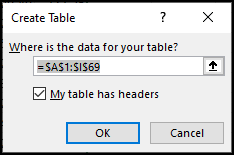
\includegraphics[width=\maxwidth{.95\linewidth}]{gfx/ch09_fig10}
		\caption{Creating a Data Table}
		\label{09:fig10}
	\end{figure}
	
	\item Click \fmtPopupButton{OK}.
\end{enumerate}

Excel creates a data table (Figure \ref{09:fig11}), which has many of the properties expected of a database. 

\begin{figure}[H]
	\centering
	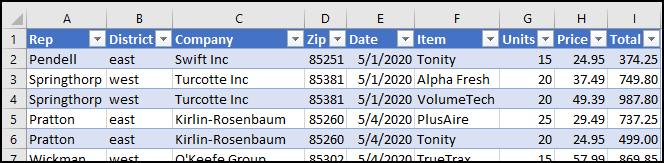
\includegraphics[width=\maxwidth{.95\linewidth}]{gfx/ch09_fig11}
	\caption{Top Of the Data Table}
	\label{09:fig11}
\end{figure}

\begin{enumerate}[resume]
	\item At \fmtRibbonButton{Table Design $ \Rightarrow $ Properties $ \Rightarrow $ Table Name} enter \fmtTyping{Sales} as the new table name. That name is entered in a text box near the left edge of the ribbon.
\end{enumerate}

In a database, columns are referred to as ``Fields'' and rows as ``Records.'' Notice that each of the fields in the data table includes a drop-down arrow. That opens a menu with filtering functions that can be applied to the database. Figure \ref{09:fig12} illustrates the filter for the \textit{Item} field.

\begin{figure}[H]
	\centering
	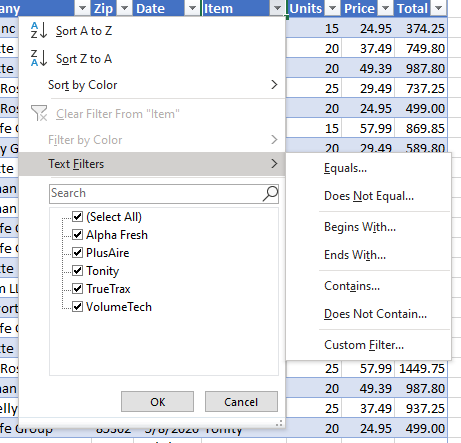
\includegraphics[width=\maxwidth{.95\linewidth}]{gfx/ch09_fig12}
	\caption{Item Filter}
	\label{09:fig12}
\end{figure}

The database can be sorted on the item field by clicking either of the top two buttons in the filter drop-down (named ``Sort A to Z'' and ``Sort Z to A''). Clicking the \fmtPopupButton{Text Filters} button opens a submenu where powerful filters can be created. Also, the checkboxes at the bottom of the popup can be used to hide or view records that match the selected item. Thus, to only see the ``Alpha Fresh'' records, uncheck all boxes except that one.

\subsection{The Database Functions}

Along with simple sorting and filtering, Excel provides the following functions that are designed to be used with a database. 

\begin{itemize}
	\item \textbf{DAVERAGE}. Calculates the average of values in a field that satisfy specified conditions.
	\item \textbf{DCOUNT}. Returns the number of cells containing numbers in a field that satisfy specified conditions.
	\item \textbf{DCOUNTA}. Returns the number of non-blank cells in a field that satisfy specified conditions.
	\item \textbf{DGET}. Returns a single value from a field that satisfy specified conditions.
	\item \textbf{DMAX}. Returns the maximum value from a field that satisfy specified conditions.
	\item \textbf{DMIN}. Returns the minimum value from a field that satisfy specified conditions.
	\item \textbf{DPRODUCT}. Calculates the product of values in a field that satisfy specified conditions.
	\item \textbf{DSTDEV}. Calculates the standard deviation (based on a sample of a population) of values in a field that satisfy specified conditions.
	\item \textbf{DSTDEVP}. Calculates the standard deviation (based on an entire population) of values in a field that satisfy specified conditions.
	\item \textbf{DSUM}. Calculates the sum of values in a field that satisfy specified conditions.
	\item \textbf{DVAR}. Calculates the variance (based on a sample of a population) of values in a field that satisfy specified conditions.
	\item \textbf{DVARP}. Calculates the variance (based on an entire population) of values in a field that satisfy specified conditions.
\end{itemize}

These functions all use similar syntax: \fmtTyping{=FuncName(Database, Field, Criteria)}. In the function, the ``FuncName'' is the name of the function, like ``DSUM.'' The database name will be ``Sales'' since that is the name of the table. The Field is one of the field names, like ``Rep'' or ``District.'' Finally, the criteria is a range that contains the factors that limit the output of the function. This is best explained with some examples.

\begin{enumerate}[resume]
	\item Enter \fmtTyping{Zip} in \fmtCellLocation{K2}, \fmtTyping{85260} in \fmtCellLocation{K3}, and \fmtTyping{Sum} in \fmtCellLocation{L3}. This will set up an area where the sum of all orders sent to Zip $ 85260 $ will be calculated.
	\item Enter this formula in \fmtCellLocation{L3}: \fmtTyping{=DSUM(Sales[\#All],''Total'',K2:K3)}. Here is what the various parts of this formula mean.

	\begin{itemize}
		\item \textbf{DSUM}. This is the ``data sum'' function that totals all of the specified data.
		\item \textbf{Sales[\#All]}. This instructs Excel to use the entire Sales data table. By using this nomenclature rather than specific cell locations (like \fmtCellLocation{A1:I69}), the formula will continue to work even if records are added to or removed from the table.
		\item \textbf{Total}. This is the field that contains the numbers to be summed. Notice that the field name is put in quote marks.
		\item \textbf{K2:K3}. This is the location of the criteria Excel will use to sum the sales amounts.
	\end{itemize}	

	\begin{figure}[H]
		\centering
		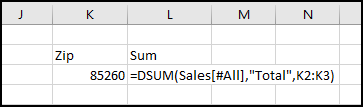
\includegraphics[width=\maxwidth{.95\linewidth}]{gfx/ch09_fig21}
		\caption{Setting Up the Data File Calculation}
		\label{09:fig21}
	\end{figure}

	\item Once the formula and criteria are entered, Excel calculates the total value of sales to that Zip and displays $ 14747.55 $.
	\item Change the Zip in \fmtCellLocation{K3} to \fmtTyping{85251}. The value in cell \fmtCellLocation{L3} will be automatically updated to $ 748.50 $, which is the total value in sales to that Zip code.
	\item Copy/paste cells \fmtCellLocation{K2:L3} to \fmtCellLocation{K5:L6}. When pasted, Excel will automatically update the criteria range in the formula to \fmtCellLocation{K5:K6}.
	\item Change the value of \fmtCellLocation{K5} to \fmtTyping{District} and \fmtCellLocation{K6} to \fmtTyping{east}. \fmtCellLocation{L6} now displays $ 22546.95 $, which is the total value of sales to the ``east'' district.
	\item Copy/paste \fmtCellLocation{K5:L6} to \fmtCellLocation{K8:L9}.
	\item Change the formula in \fmtCellLocation{L9} to calculate the average value of the total sales by changing \fmtTyping{DSUM} to \fmtTyping{DAVERAGE}. The formula in \fmtCellLocation{L9} should now be: \fmtTyping{=DAVERAGE(Sales[\#All],''Total'',K8:K9)}
	\item Change \fmtCellLocation{K8} to \fmtTyping{Rep} and \fmtCellLocation{K9} to \fmtTyping{Pratton}. \fmtCellLocation{L9} should now display $ 736.7236842 $, which is the average sale value for Pratton. The average sale for other sellers can be easily checked by entering their names in \fmtCellLocation{K9}, one at a time.
\end{enumerate}

One important feature for any database lookup is the ability to specify ``Boolean'' matches; that is, a match that includes an AND term or an OR term. For example, that would answer a question like, ``What is the total value of the sales of TrueTrax made by Findlay?'' Follow these steps to create Boolean expressions.

\begin{enumerate}
	\item Copy/paste \fmtCellLocation{K8:K9} to \fmtCellLocation{K11:K12} and also paste \fmtCellLocation{K8:K9} to \fmtCellLocation{L8:L9}. Change \fmtCellLocation{K11} to \fmtTyping{Rep}, \fmtCellLocation{K12} to \fmtTyping{Findlay}, \fmtCellLocation{L11} to \fmtTyping{Item} and \fmtCellLocation{L12} to \fmtTyping{TrueTrax}.
	\item Copy/paste \fmtCellLocation{L8:L9} to \fmtCellLocation{M11:M12}. Change the formula in \fmtCellLocation{M12} to \fmtTyping{=DSUM(Sales[\#All],''Total'',K11:L12)}.
	
	\begin{figure}[H]
		\centering
		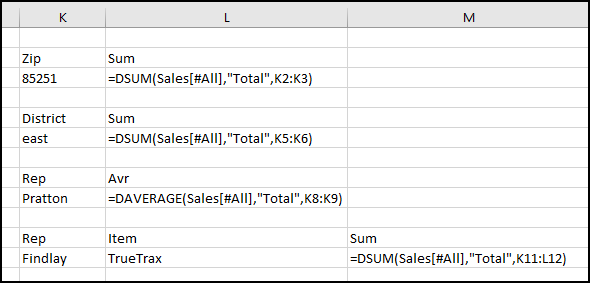
\includegraphics[width=\maxwidth{.95\linewidth}]{gfx/ch09_fig22}
		\caption{Calculating an AND Expression}
		\label{09:fig22}
	\end{figure}
	
	\item Excel displays $ 1739.7 $ in \fmtCellLocation{M12}, which is the total value of Findlay's TrueTrax sales. 
	\item Data criteria items that appear in the same row are combined with an AND, so K11:L12 would be read ``Calculate the sum of all lines that include a representative named Findlay AND an item named TrueTrax.''
	\item Note: The order of the ANDed terms is important. They must be in the same order in the criteria section as they are in the data table. Therefore, if ``Item'' were in \fmtCellLocation{K11} and ``Rep'' in \fmtCellLocation{L11} the formula would fail.
	\item Other sales representative names can be entered in cell \fmtCellLocation{K12} or other items in \fmtCellLocation{L12} to check on those sales.
	\item To combine two or more terms with an OR, place those terms on separate lines. 
	\item Copy/paste \fmtCellLocation{K11:M12} to \fmtCellLocation{K14:M15}.
	\item Rather than calculate the total value of Findlay's sales, count the number of items sold. Change \fmtCellLocation{M14} to \fmtTyping{Units Sold}.
	\item Change the formula in \fmtCellLocation{M15} to: \fmtTyping{=DSUM(Sales[\#All],''Units'',K14:L15)}. Notice that the only change to the formula is that it will sum the \textit{Units} field instead of the \textit{Total} field.
	\item To include PlusAir in this sum, enter \fmtTyping{PlusAir} in \fmtCellLocation{L16}. Then, change the formula in \fmtCellLocation{M15} to \fmtTyping{=DSUM(Sales[\#All],''Units'',K14:L16)}. Notice that the only change is to increase the criteria range to \fmtCellLocation{K14:L16}. Now, Excel will count the total number of lines that include both Findlay and TrueTrax OR Finaley and PlusAir. Excel reports that Findlay sold $ 50 $ TrueTrax OR PlusAir units.
	
	\begin{figure}[H]
		\centering
		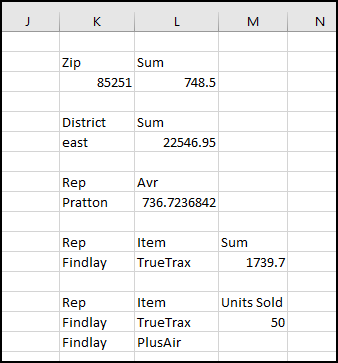
\includegraphics[width=\maxwidth{.95\linewidth}]{gfx/ch09_fig23}
		\caption{Calculating an OR Expression}
		\label{09:fig23}
	\end{figure}
\end{enumerate}

Finally, it is often desirable to set up a range for a data calculation. For example, it is possible to count the total number of Tonity sales made between May $ 5 $ and May $ 20 $.

\begin{enumerate}
	\item Enter \fmtTyping{Date} in \fmtCellLocation{K18}, \fmtTyping{Date} in \fmtCellLocation{L18} (the Date will be entered two times in the criteria), \fmtTyping{Item} in \fmtCellLocation{M18}, and \fmtTyping{Count} in \fmtCellLocation{N18}.
	\item Enter \fmtTyping{$>$=5/10/2020} in \fmtCellLocation{K19}, \fmtTyping{$<$=5/20/2020} in \fmtCellLocation{L19}, and \fmtTyping{Tonity} in \fmtCellLocation{M19}.
	\item Enter this formula in \fmtCellLocation{N19}: \fmtTyping{=DCOUNT(Sales[\#All],''Total'',K18:M19)}. Notice that this is a DCOUNT formula, so the number of lines that contain a Tonity item sold between $ 5/10/2020 $ and $ 5/20/2020 $ (inclusive) will be counted.
	
	\begin{figure}[H]
		\centering
		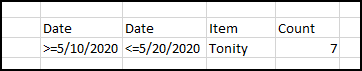
\includegraphics[width=\maxwidth{.95\linewidth}]{gfx/ch09_fig24}
		\caption{Specifying a Date Range}
		\label{09:fig24}
	\end{figure}

	\item Excel reports seven Tonity sales were made between the two specified dates.

\end{enumerate}

Creating a data table is easy in Excel, then the data formulas make it easy to create complex calculations by simply specifying the criteria.
	
\begin{center}
	\begin{tkwbox}{Key Take-Aways}
		\textbf{Database Functions}
		\\
		\begin{itemize}
			\setlength{\itemsep}{0pt}
			\setlength{\parskip}{0pt}
			\setlength{\parsep}{0pt}
			
			\item Set up the database functions by creating a data table.
			\item Use any of the ``D...'' functions to easily count, sum, or statistically analyze a data table using complex Boolean operations. 
			
		\end{itemize}
	\end{tkwbox}
\end{center}

\section{Useful Functions}

\begin{center}
	\begin{objbox}{Learning Objectives}
		\begin{itemize}
			\setlength{\itemsep}{0pt}
			\setlength{\parskip}{0pt}
			\setlength{\parsep}{0pt}
			
			\item Practice with $ 8 $ of Excel's most useful text functions.
			\item Practice with $ 12 $ of Excel's most useful numeric functions.
			
		\end{itemize}
	\end{objbox}
\end{center}

Excel includes more than $ 300 $ functions that are designed to process both text and numbers. The vast majority of those functions are only useful in specific situations and most users will never know that they exist; however, many functions are so commonly used that they show up in many spreadsheet projects. This section provides information and practice with $ 20 $ of the most useful functions.

A contact roster will be used for the exercises in this section. This file contains information that would be used by sales representatives as they work with a company's clients. The roster needs to be cleaned up a bit for more efficient use. (Note: the roster contains fake data.)

\begin{enumerate}
	\item Open workbook \fmtWorkbookName{CH9-ContactData.xlsx}
	\item This workbook has only one worksheet, \fmtWorksheetName{Contacts}.
	\item Save the workbook as \fmtWorkbookName{CH9-Contact.xlsx}.
\end{enumerate}

\subsection{Text Functions}

Excel includes scores of functions designed to be used with cells that contain text rather than numbers and this section explores the most commonly-used text functions.

\subsubsection{To Columns}

Often, a field in a data file contains two or more separate pieces of information. This makes it impossible to complete tasks like sorting on the individual pieces of information. The Name data field (\fmtCellLocation{Column B}) in the \fmtWorksheetName{Contacts} worksheet includes both first and last names, but those should be placed in different fields. This is such a common operation, Excel has a function that splits data separated by a comma into two different fields.

\begin{enumerate}
	\item Insert a new column to the left of \fmtCellLocation{Column C}. This column will eventually contain the first name and \fmtCellLocation{Column B} will contain the last name.
	\item Click \fmtCellLocation{B2} and then shift-click \fmtCellLocation{B101} to highlight all of the data in \fmtCellLocation{Column B}.
	\item Click \fmtRibbonButton{Data $ \Rightarrow $ Data Tools $ \Rightarrow $ Text to Columns}.
	\item Excel starts a data wizard to help split the data. The first screen is used to adjust from delimited to fixed width data type, but the default, delimited, is correct, so click \fmtPopupButton{Next}.
	
	\begin{figure}[H]
		\centering
		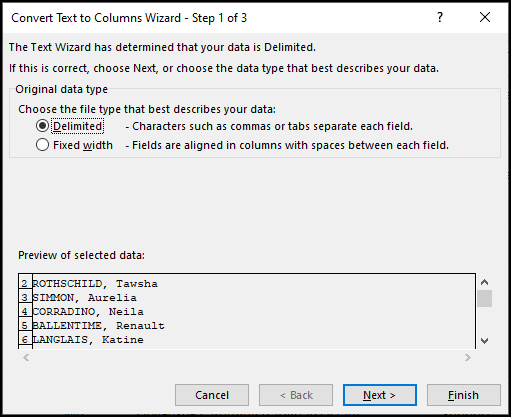
\includegraphics[width=\maxwidth{.95\linewidth}]{gfx/ch09_fig30}
		\caption{Convert Text to Columns Wizard Screen 1}
		\label{09:fig30}
	\end{figure}

	\item The second wizard box determines what sort of delimiter is used with the data. For this field, the first and last names are separated by a comma, so check the \fmtPopupButton{Comma} delimiter and uncheck the \fmtPopupButton{Tab} delimiter. The sample data at the bottom of the Wizard screen should show the first and last names properly divided. Click \fmtPopupButton{Next}.

	\begin{figure}[H]
		\centering
		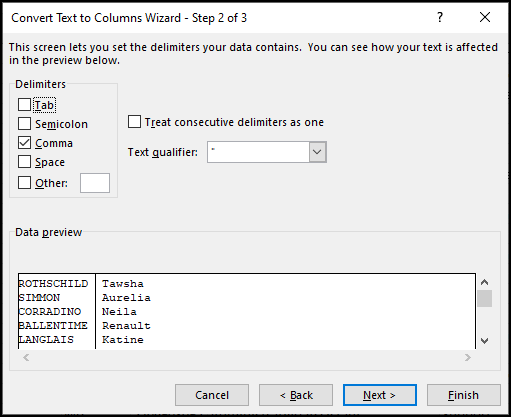
\includegraphics[width=\maxwidth{.95\linewidth}]{gfx/ch09_fig31}
		\caption{Convert Text to Columns Wizard Screen 2}
		\label{09:fig31}
	\end{figure}

	\item The third wizard box determines the type of data each column contains. Since the default, \textit{General}, is appropriate, click \fmtPopupButton{Finish}.

	\begin{figure}[H]
		\centering
		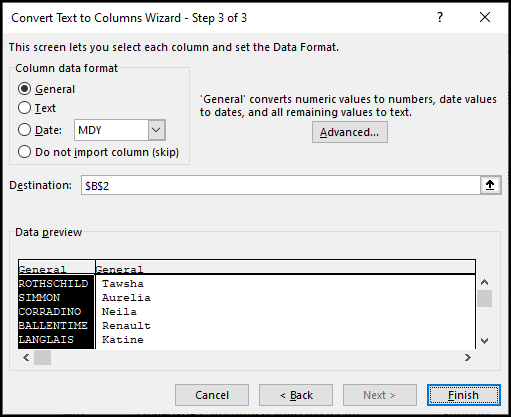
\includegraphics[width=\maxwidth{.95\linewidth}]{gfx/ch09_fig32}
		\caption{Convert Text to Columns Wizard Screen 3}
		\label{09:fig32}
	\end{figure}

	\item Excel splits the names into two colums. 
	\item Click \fmtCellLocation{B1} and enter \fmtTyping{Last\_Name}.
	\item Click \fmtCellLocation{C1} and enter \fmtTyping{First\_Name}.
	\item Adjust \fmtCellLocation{Column B} and \fmtCellLocation{Column C} so they are the optimum width.
	
	\begin{figure}[H]
		\centering
		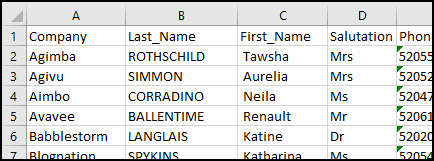
\includegraphics[width=\maxwidth{.95\linewidth}]{gfx/ch09_fig33}
		\caption{Names Divided Into Two Columns}
		\label{09:fig33}
	\end{figure}
\end{enumerate}

\subsubsection{Trim}

\[ =TRIM(text) \]

The \textit{Trim} function is used to trim unwanted spaces from the start or end of text in a cell.

\begin{enumerate}
	\item This excercise uses the \fmtWorksheetName{Contacts} worksheet in the \fmtWorkbookName{Contact} workbook.
	\item When the name was separated into Last and First name columns, Excel automatically added a space at the start of the First Name field. That space, though, will be a problem in later exercises. 
	\item Insert a new column to the left of \fmtCellLocation{Column D}. The newly-inserted column becomes \fmtCellLocation{Column D}.
	\item Enter this formula in \fmtCellLocation{D2}: \fmtTyping{=trim(C2)}
	\item Copy \fmtCellLocation{D2} to \fmtCellLocation{D3:D101}. This removes the leading space from the first names.
	\item Select and copy \fmtCellLocation{D2:D101}.
	\item Paste Values to \fmtCellLocation{C2:C101}. Note: it is important to paste the values, not just a simple paste. Otherwise, \fmtCellLocation{C2:C101} will be filled with the \textit{trim} formula rather than the value generated by that formula.
	
	\begin{figure}[H]
		\centering
		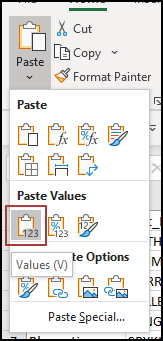
\includegraphics[width=\maxwidth{.95\linewidth}]{gfx/ch09_fig34}
		\caption{Paste Values Button}
		\label{09:fig34}
	\end{figure}
	
	\item Delete \fmtCellLocation{Column D}.
	\item Though it is not visible, the data in \fmtCellLocation{Column F} (the ``Role'' column) has a random number of spaces trailing many of the entries, which is a common problem caused by sloppy data entry.
	\item Insert a new column to the left of \fmtCellLocation{Column G}. The newly-inserted column becomes \fmtCellLocation{Column G}.
	\item Enter this formula in \fmtCellLocation{G2}: \fmtTyping{=trim(F2)}
	\item Copy \fmtCellLocation{G2} to \fmtCellLocation{G3:G101}. This removes the trailing space from all entries in the role data.
	\item Select and copy \fmtCellLocation{G2:G101}.
	\item Paste Values to \fmtCellLocation{F2:F101}. Note: it is important to paste the values, not just a simple paste. Otherwise, \fmtCellLocation{F2:F101} will be filled with the \textit{trim} formula rather than the value generated by that formula.
	\item Delete \fmtCellLocation{Column G}.
\end{enumerate}

\subsubsection{Upper/Lower/Proper}

\[ =UPPER(text) \]
\[ =LOWER(text) \]
\[ =PROPER(text) \]

Often, the text case needs to be changed. The \textit{upper} function changes text to upper case, the \textit{lower} function changes text to lower case, and the \textit{proper} function changes to title case (the first letter of each word is capitalized). 

\begin{enumerate}
	\item This excercise uses the \fmtWorksheetName{Contacts} worksheet in the \fmtWorkbookName{Contact} workbook.
	\item For some reason, the last names in \fmtCellLocation{Column B} are uppercase. Uppercase text is commonly found, but that type of text is difficult to read.
	\item Insert a new column to the left of \fmtCellLocation{Column C}. The newly-inserted column becomes \fmtCellLocation{Column C}.
	\item Enter this formula in \fmtCellLocation{C2}: \fmtTyping{=proper(B2)}
	\item Copy \fmtCellLocation{C2} to \fmtCellLocation{C3:C101}. This changes the last names to proper case.
	\item Select and copy \fmtCellLocation{C2:C101}.
	\item Paste Values to \fmtCellLocation{B2:B101}. Note: it is important to paste the values, not just a simple paste. Otherwise, \fmtCellLocation{B2:B101} will be filled with the \textit{proper} formula rather than the value generated by that formula.
	\item Delete \fmtCellLocation{Column C}.
\end{enumerate}

\subsubsection{Left/Right/Mid}

\[ =LEFT(text, [num\_chars]) \]
\[ =RIGHT(text, [num\_chars]) \]
\[ =MID(text, start\_num, [num\_chars]) \]

The \textit{left}, \textit{right}, and \textit{mid} functions are used to extract letters from a text field. For example, Cell \fmtCellLocation{B2} contains \textit{Rothschild}. The function \fmtTyping{=left(B2,4)} would extract ``Roth,'' the left four letters in that field. The function \fmtTyping{=right(B2,5)} would extract ``child,'' the right five letters in that field. The function \fmtTyping{=mid(B2,5,3)} would extract ``sch,'' the three letters starting in position five in that field. These functions, along with \textit{concatenate} in the next section, are used to change the format of the phone number (\fmtCellLocation{Column E})from ten digits to (xxx) xxx-xxxx.

\subsubsection{Concatenate}

\[ =CONCATENATE(text1, text2, [text3], ...) \]

Frequently, text stored in various workbook cells needs to be combined to create new information. The \textit{concatenate} function makes this possible. The various text phrases to combine are entered one after another, separated by commas. This exercise uses \textit{concatenate} along with \textit{left}, \textit{right}, and \textit{mid} to change the format of the phone number from ten digits to (xxx) xxx-xxxx.

\fmtExcelNew{365} Note: this function was renamed \textit{concat} in Excel $ 365 $.

\begin{enumerate}
	\item This excercise uses the \fmtWorksheetName{Contacts} worksheet in the \fmtWorkbookName{Contact} workbook.
	\item Insert a new column to the left of \fmtCellLocation{Column F}. The newly-inserted column becomes \fmtCellLocation{Column F}.
	\item Enter this formula in \fmtCellLocation{F2}: \fmtTyping{=CONCATENATE("(",LEFT(E2,3),") ",MID(E2,4,3),"-",RIGHT(E2,4))}
	\item Copy \fmtCellLocation{F2} to \fmtCellLocation{F3:F101}. This changes the format of the phone number to (xxx) xxx-xxxx.
	\item Select and copy \fmtCellLocation{F2:F101}.
	\item Paste Values to \fmtCellLocation{E2:E101}. Note: it is important to paste the values, not just a simple paste. Otherwise, \fmtCellLocation{E2:E101} will be filled with the \textit{concatenate} formula rather than the value generated by that formula.
	\item Delete \fmtCellLocation{Column F}.
	\item Adjust the width of \fmtCellLocation{Column E} to properly display the formatted phone number.
\end{enumerate}

\subsubsection{Search}	

\[ =SEARCH(find\_text, within\_text, [start\_num]) \]

The \textit{search} function is used to find a phrase in a cell that contains text. This is similar to the \textit{left}/\textit{right}/\textit{mid} functions except with \textit{search} the exact starting position of the target data is not known in advance. Therefore, \textit{search} could be used to find the phrase ``good'' in strings like ``good morning'' and ``the greater good'' where the target phrase starts in different locations in each string. Optionally, a specific start point for the search can be specified. Search returns the position where the target phrase starts, so search would report that ``good'' in ``good morning'' starts at position one but in ``the greater good'' it starts at position $ 13 $. For this exercise, the year needs to be extracted from the \textit{Contract\_Num} field (\fmtCellLocation{Column J}). The starting position for the year varies so \textit{search} is needed instead of a simple \textit{left/right/mid} function. Note: \textit{search} is not case sensitive but the Excel function \textit{find} is case sensitive. Other then that, the two functions are identical. Thus, to find ``Good'' in a cell, use \textit{search} if the capital letter should be ignored but \textit{find} if the capital letter is important.

\begin{enumerate}
	\item This excercise uses the \fmtWorksheetName{Contacts} worksheet in the \fmtWorkbookName{Contact} workbook.
	\item Insert a new column to the left of \fmtCellLocation{Column K}. The newly-inserted column becomes \fmtCellLocation{Column K}.
	\item Enter \fmtTyping{Year} in \fmtCellLocation{K1}. This column will contain the extracted year.
	\item Enter this formula in \fmtCellLocation{K2}: \fmtTyping{=VALUE(MID(J2, SEARCH("-", J2)+1,4))}. This is a complex formula, but it can be broken down like this: 
	
	\begin{itemize}
		\item \textbf{SEARCH(``-'',J2)}. Search for a hyphen in data field \fmtCellLocation{J2}.
		\item \textbf{MID(J2, SEARCH("-", J2)+1,4)}. Using the MID function, extract from data field \fmtCellLocation{J2}, starting one letter past the position of the hyphen, for four characters.
		\item \textbf{=VALUE(MID(J2, SEARCH("-", J2)+1,4))}. Convert the extracted text to a number rather than store it as text. Note: Excel would store an extracted phrase as text, but since these are years it is sensible to store them as numbers so various statistical functions can later be used.
	\end{itemize}

	\item Copy \fmtCellLocation{K2} to \fmtCellLocation{K3:K101}. This finds the year from each of the contract numbers.
	\item Select and copy \fmtCellLocation{K2:K101}.
	\item Paste Values to \fmtCellLocation{K2:K101}. Note: it is important to paste the values, not just a simple paste. This looks odd since the cells are being pasted back into the same locations from which they were copied, but this is a good way to remove a formula from a cell without creating an additional data column.
	\item Adjust the width of \fmtCellLocation{Column K} to optimally fit the year data.
	
	\begin{figure}[H]
		\centering
		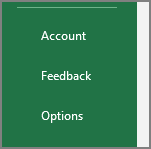
\includegraphics[width=\maxwidth{.95\linewidth}]{gfx/ch09_fig35}
		\caption{Extracting the Year from the Contract Number}
		\label{09:fig35}
	\end{figure}
	
\end{enumerate}

\subsubsection{VLookup}

\[ =VLOOKUP(value, table, col\_index, [approx]) \]

\textit{VLookup} is one of the most useful, and complex, Excel functions. It is used to lookup and return a value from a table. \textit{VLookup} will look up the value in column one of a specified data range and return the value from the indexed column number. This concept is much easier to understand with an example. Consider Table \ref{09:tab01}.

\begin{table}[H]
	\rowcolors{1}{}{tablerow} % zebra striping background
	{\small
		%\fontsize{8}{10} \selectfont %Replace small for special font size
		\begin{longtable}{L{0.30in}L{0.50in}L{1.00in}L{0.50in}} %Left-aligned, Max width: 4.25in
			\textbf{ID} & \textbf{Name} & \textbf{Phone} & \textbf{Section} \endhead
			\hline
			0134 & Jones & (520) 123-4567 & Sales\\
			0293 & Marks & (520) 398-2219 & HR\\
			0342 & Nash  & (520) 721-9043 & Orders\\
			\rowcolor{captionwhite}
			\caption{VLookup Example Table}
			\label{09:tab01}
		\end{longtable}
	} % End small
\end{table}

The formula \fmtTyping{=VLOOKUP(0293,A2:D5,2)} would return ``Marks'' because that is the value stored in the second column of the table for the row that starts with ``0293.''

The last item in the VLOOKUP function, ``approx,'' determines if the match in column can be approximate or if an exact match is required. If the value for this item is TRUE then an approximate match is acceptable (this is the default), but if it is FALSE then the match must be exact. 

\begin{enumerate}
	\item This excercise uses the \fmtWorksheetName{Contacts} worksheet in the \fmtWorkbookName{Contact} workbook.
	\item In cell \fmtCellLocation{P3} enter \fmtTyping{Company}.
	\item In cell \fmtCellLocation{P4} enter \fmtTyping{Last Name}.
	\item In cell \fmtCellLocation{P5} enter \fmtTyping{Phone}.
	\item In cell \fmtCellLocation{P6} enter \fmtTyping{Role}.
	\item In cell \fmtCellLocation{Q3} enter \fmtTyping{Agimba}. This is the name of the first company, found in cell \fmtCellLocation{A2}.
	\item In cell \fmtCellLocation{Q4} enter \fmtTyping{=VLOOKUP(\$Q\$2,\$A\$1:\$F\$101,2,FALSE)}. This formula will lookup the company found in cell \fmtCellLocation{Q3}, ``Agimba,'' in column one of the table found in \fmtCellLocation{A1:F101} and then return the value found in column two of that table. When completed, cell \fmtCellLocation{Q4} should contain ``Rothschild,'' which is the name of the representative at Agimba. Notice that the formula uses absolute references so if it is copied to other cells it will still refer to the correct table. Also notice that the last item in the formula is ``FALSE'' which makes Excel look for an exact match rather than an approximate match.
	\item In cell \fmtCellLocation{Q5} enter \fmtTyping{=VLOOKUP(\$Q\$2,\$A\$1:\$F\$101,5,FALSE)}. This formula will lookup the company found in cell \fmtCellLocation{Q3}, ``Agimba,'' in column one of the table found in \fmtCellLocation{A2:F101} and then return the value found in column five of that table. When completed, cell \fmtCellLocation{Q5} should contain ``(520) 555-1082,'' which is Agimba's phone number.  Notice that the formula uses absolute references so if it is copied to other cells it will still refer to the correct table. Also notice that the last item is ``FALSE'' which makes Excel look for an exact match rather than an approximate match.
	\item In cell \fmtCellLocation{Q6} enter \fmtTyping{=VLOOKUP(\$Q\$2,\$A\$1:\$F\$101,6,FALSE)}. This formula will lookup the company found in cell \fmtCellLocation{Q3}, ``Agimba,'' in column one of the table found in \fmtCellLocation{A2:F101} and then return the value found in column six of that table. When completed, cell \fmtCellLocation{Q6} should contain ``Business Analyst,'' which is the role of the contact at Agimba.  Notice that the formula uses absolute references so if it is copied to other cells it will still refer to the correct table. Also notice that the last item is ``FALSE'' which makes Excel look for an exact match rather than an approximate match.
	
	\begin{figure}[H]
		\centering
		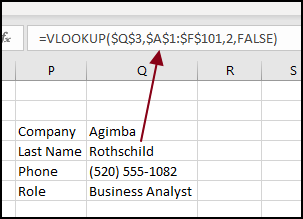
\includegraphics[width=\maxwidth{.95\linewidth}]{gfx/ch09_fig36}
		\caption{VLookup Formula for Q4}
		\label{09:fig36}
	\end{figure}
	
	\item If the company in cell \fmtCellLocation{Q3} is changed then the data displayed in \fmtCellLocation{Q4:Q6} will be updated to match the new name. Try entering \fmtTyping{Blogtag} and \fmtTyping{Eidel} in \fmtCellLocation{Q3} to check the update feature.
\end{enumerate}

\subsubsection{Index Match}

\[ =INDEX(data,MATCH(value,lookup\_column,FALSE),column) \]

This is the most complex formula in this book and is a combination of two simpler functions: \textit{index} and \textit{match}. On the surface, it does almost exactly what \textit{VLookup} does, so many people do not bother to learn the \textit{Index Match} formula. However, \textit{VLookup} requires the lookup field to be in column one of the data table while \textit{Index Match} can look up data in any column. Also, if the data table is changed in some way (a new column added, for example), \textit{VLookup} will no longer work but \textit{Index Match} will be adapt to the new table structure. So the time taken to learn this lookup formula will result in a more robust lookup function.

\begin{enumerate}
	\item This excercise uses the \fmtWorksheetName{Contacts} worksheet in the \fmtWorkbookName{Contact} workbook.
	\item In cell \fmtCellLocation{P8} enter \fmtTyping{Contract Num}.
	\item In cell \fmtCellLocation{P9} enter \fmtTyping{Company}.
	\item In cell \fmtCellLocation{P10} enter \fmtTyping{Phone}.
	\item In cell \fmtCellLocation{P11} enter \fmtTyping{Last Name}.
	\item In cell \fmtCellLocation{Q8} enter \fmtTyping{Agim(BusDev)-2013-21}. This is the contract number for the first data row, found in cell \fmtCellLocation{J2}.
	\item In cell \fmtCellLocation{Q9} enter \fmtTyping{=INDEX(\$A\$2:\$F\$101,MATCH(\$Q\$8,\$J\$2:\$J\$101,FALSE),1)}. This is a complex formula and it will help to break it down into smaller chunks. 
	
	\begin{itemize}
		\item \textbf{MATCH(\$Q\$8,\$J\$2:\$J\$101,FALSE)}. In the center of the complex formula is a \textit{MATCH} function. That will look for the value in cell \fmtCellLocation{Q8} (the contract number) in \fmtCellLocation{J2:J101} (the contract data field). An exact match is required since the last parameter is FALSE. If the contract number is found then MATCH will return the row number for that contract.
		\item \textbf{=INDEX(\$A\$2:\$F\$101,RowNum,1)}. \textit{INDEX} will use the row number (\textit{RowNum}) returned by the \textit{MATCH} function and return the data in column one (Company name) of the data table in \fmtCellLocation{A2:F101}.
	\end{itemize}
		
	\item When completed, cell \fmtCellLocation{Q9} should contain ``Agimba,'' which is the name of the company for the contract number in cell \fmtCellLocation{Q8}. Notice that the formula uses absolute references so if it is copied to other cells it will still refer to the correct table.
	\item In cell \fmtCellLocation{Q10} enter \fmtTyping{=INDEX(\$A\$2:\$F\$101,MATCH(\$Q\$8,\$J\$2:\$J\$101,FALSE),5)}. This formula will match the contract number found in cell \fmtCellLocation{Q8} and then return the value found in column five of the data table. When completed, cell \fmtCellLocation{Q10} should contain ``(520) 555-1082,'' which is the phone number for the company.  Notice that the formula uses absolute references so if it is copied to other cells it will still refer to the correct table. 
	\item In cell \fmtCellLocation{Q11} enter \fmtTyping{=INDEX(\$A\$2:\$F\$101,MATCH(\$Q\$8,\$J\$2:\$J\$101,FALSE),2)}. This formula will lookup the contract number found in cell \fmtCellLocation{Q8} and then return the value found in column two of the data table. When completed, cell \fmtCellLocation{Q11} should contain ``Rothschild,'' which is the last name of the contact for this contract.  Notice that the formula uses absolute references so if it is copied to other cells it will still refer to the correct table. 
	
	\begin{figure}[H]
		\centering
		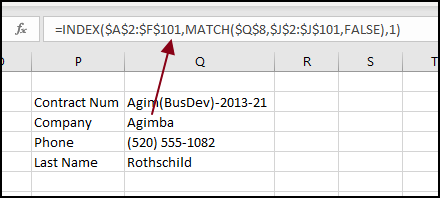
\includegraphics[width=\maxwidth{.95\linewidth}]{gfx/ch09_fig37}
		\caption{Index-Match Formula for Q9}
		\label{09:fig37}
	\end{figure}
	
	\item If the name in contract number in \fmtCellLocation{Q8} is changed then the data displayed in \fmtCellLocation{Q9:Q11} will be updated to match the new number. Try entering \fmtTyping{Buzz(Sales)-2014-117} and \fmtTyping{Link(RD)-2013-21} in \fmtCellLocation{Q8} to check the update feature.
		
\end{enumerate}

\subsection{Number Functions}

Excel has hundreds of functions designed to be used with cells that contain numbers and this section explores the most commonly-used number functions.

\subsubsection{Sum}

\[ =SUM(number1, [number2], [number3], ...) \]

This function adds all of the values in a specified range. 

\begin{enumerate}
	\item This excercise uses the \fmtWorksheetName{Contacts} worksheet in the \fmtWorkbookName{Contact} workbook.
	\item Enter \fmtTyping{Total Value} in cell \fmtCellLocation{P13}.
	\item Enter this formula into \fmtCellLocation{Q13}: \fmtTyping{=SUM(L2:L101)}. This formula will total all of the contract values found in \fmtCellLocation{Column L}.
	\item When completed, cell \fmtCellLocation{Q13} should contain $ 4374391 $. This number could be formatted with Excel's formatting tools to be easier to read.

	\begin{figure}[H]
		\centering
		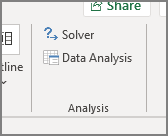
\includegraphics[width=\maxwidth{.95\linewidth}]{gfx/ch09_fig38}
		\caption{Sum Formula for Q13}
		\label{09:fig38}
	\end{figure}
	
\end{enumerate}

\subsubsection{Average}

\[ =AVERAGE(number1, [number2], [number3], ...) \]

This function calculates the average for the values in a specified range. 

\begin{enumerate}
	\item This excercise uses the \fmtWorksheetName{Contacts} worksheet in the \fmtWorkbookName{Contact} workbook.
	\item Enter \fmtTyping{Average Value} in cell \fmtCellLocation{P14}.
	\item Enter this formula into \fmtCellLocation{Q14}: \fmtTyping{=AVERAGE(L2:L101)}. This formula will calculate the average of the contract values found in column L.
	\item When completed, cell \fmtCellLocation{Q14} should contain $ 43743.91 $. This number could be formatted with Excel's formatting tools to be easier to read.

	\begin{figure}[H]
		\centering
		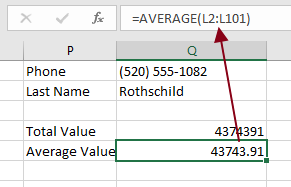
\includegraphics[width=\maxwidth{.95\linewidth}]{gfx/ch09_fig39}
		\caption{Average Formula for Q14}
		\label{09:fig39}
	\end{figure}

\end{enumerate}

\subsubsection{Min/Max}

\[ =MIN(number1, [number2], [number3], ...) \]
\[ =MAX(number1, [number2], [number3], ...) \]

These functions find the minimum or maximum value in a specified range. 

\begin{enumerate}
	\item This excercise uses the \fmtWorksheetName{Contacts} worksheet in the \fmtWorkbookName{Contact} workbook.
	\item Enter \fmtTyping{Max Value} in cell \fmtCellLocation{P15}.
	\item Enter this formula into \fmtCellLocation{Q15}: \fmtTyping{=MAX(L2:L101)}. This formula will find the maximum contract value in column L.
	\item When completed, cell \fmtCellLocation{Q15} should contain $ 88050 $.
	\item Enter \fmtTyping{Min Value} in cell \fmtCellLocation{P16}.
	\item Enter this formula into \fmtCellLocation{Q16}: \fmtTyping{=MIN(L2:L101)}. This formula will find the minimum contract value in column L.
	\item When completed, cell \fmtCellLocation{Q16} should contain $ 5140 $.

	\begin{figure}[H]
		\centering
		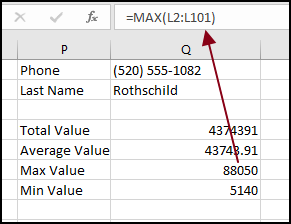
\includegraphics[width=\maxwidth{.95\linewidth}]{gfx/ch09_fig40}
		\caption{Max Formula for Q15}
		\label{09:fig40}
	\end{figure}

\end{enumerate}

\subsubsection{Round}

\[ =ROUND(number, num\_digits) \]

This function rounds a number to a specified number of digits. If the number of digits is a positive number then it will be rounded to a decimal value but if the number of digits is negative then it will be rounded to the nearest multiple of ten. Table \ref{09:tab02} will help to clarify this concept.

\begin{table}[H]
	\rowcolors{1}{}{tablerow} % zebra striping background
	{\small
		%\fontsize{8}{10} \selectfont %Replace small for special font size
		\begin{longtable}{R{0.75in}C{0.80in}R{0.60in}L{1.50in}} %Left-aligned, Max width: 4.25in
			\textbf{Number} & \textbf{Num\_Digits} & \textbf{Result} & Notes \endhead
			\hline
			5678.1234 &  3 & 5678.123 & 3 decimal places \\
			5678.1234 &  2 & 5678.12  & 2 decimal places\\
			5678.1234 &  1 & 5678.1   & 1 decimal place\\
			5678.1234 &  0 & 5678     & Nearest whole number\\
			5678.1234 & -1 & 568      & Nearest 10\\
			5678.1234 & -2 & 57       & Nearest 100\\
			5678.1234 & -3 & 6        & Nearest 1,000\\
			\rowcolor{captionwhite}
			\caption{Rounding Places}
			\label{09:tab02}
		\end{longtable}
	} % End small
\end{table}

\begin{enumerate}
	\item This excercise uses the \fmtWorksheetName{Contacts} worksheet in the \fmtWorkbookName{Contact} workbook.
	\item Enter \fmtTyping{Rounded Value} in cell \fmtCellLocation{P18}.
	\item Enter this formula into \fmtCellLocation{Q18}: \fmtTyping{=ROUND(Q13,-4)}. This formula will round the Total Value in cell \fmtCellLocation{Q13} to the nearest $ 10,000 $.
	\item When completed, cell \fmtCellLocation{Q18} should contain $ 4370000 $. This number could be formatted with Excel's formatting tools to be easier to read.
\end{enumerate}

\subsubsection{If}

\[ =IF(logical\_test, [value\_if\_true], [value\_if\_false]) \]

The \textit{IF} function fills a cell with some value based on the result of an ``if'' decision. As an example of the \textit{IF} function, a cell on the \fmtWorksheetName{Contacts} worksheet will be used to indicate if the value of a contract is greater than a specified threshold.

\begin{enumerate}
	\item This excercise uses the \fmtWorksheetName{Contacts} worksheet in the \fmtWorkbookName{Contact} workbook.
	\item Insert a new column to the left of \fmtCellLocation{Column M}. The newly-inserted column becomes \fmtCellLocation{Column M}.
	\item Enter \fmtTyping{Priority} in cell \fmtCellLocation{M1}.
	\item Adjust the width of \fmtCellLocation{Column M} to properly display cell \fmtCellLocation{M1}.
	\item Enter this formula into \fmtCellLocation{M2}: \fmtTyping{=IF(L2>50000,"High","Low")}. This formula will check the value in cell \fmtCellLocation{L2} and if it is greater than $ 50000 $ it will enter the word ``High'' in \fmtCellLocation{M2} otherwise it will enter the word ``Low.''
	\item When completed, cell \fmtCellLocation{M2} should contain ``Low.''
	\item Copy cell \fmtCellLocation{M2} to \fmtCellLocation{M3:M10}. Notice that if the value in \fmtCellLocation{Column L} is greater than $ 50000 $ then \fmtCellLocation{Column M} will display ``High,'' otherwise it will display the word ``Low.''
	\item Commonly, \textit{IF} functions are nested to get a more granular output. For this worksheet, to get a Priority (\fmtCellLocation{Column M}) of ``High,'' ``Med,'' or ``Low,'' the formula will need to be adjusted.
	\item Enter this formula into \fmtCellLocation{M2}: \fmtTyping{=IF(L2>60000,"High",IF(L2>30000,"Med","Low"))}
	
	\begin{itemize}
		\item If the value in \fmtCellLocation{L2} is greater than $ 60,000 $ then Excel will print ``High'' and be done.
		\item If the value in \fmtCellLocation{L2} is less than or equal to $ 60,000 $ then Excel will check to see if it is greater than $ 30,000 $. If so, Excel will print ``Med.''
		\item If the value in \fmtCellLocation{L2} is less than or equal to $ 30,000 $, Excel will print ``Low.''
	\end{itemize}

	\item Copy the formula in \fmtCellLocation{M2} to \fmtCellLocation{M3:M101}. Notice that some values are flagged as ``High'' priority, some as ``Med'' priority, and some as ``Low'' priority.
	
	\begin{figure}[H]
		\centering
		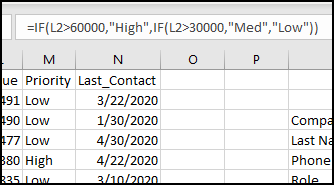
\includegraphics[width=\maxwidth{.95\linewidth}]{gfx/ch09_fig41}
		\caption{IF Formula for M2}
		\label{09:fig41}
	\end{figure}
	
\end{enumerate}

\subsubsection{SumIf/SumIfS}

\[ =SUMIF(range, criteria, [sum\_range]) \]
\[ =SUMIFS(sum\_range, range1, criteria1, [range2], [criteria2], ...) \]

These two functions will calculate a sum but only if certain specified criteria are true. The difference between the two functions is that \textit{SUMIF} can only have one criterion while \textit{SUMIFS} can have two or more criteria. Both functions are used in the following exercise.

\begin{enumerate}
	\item This excercise uses the \fmtWorksheetName{Contacts} worksheet in the \fmtWorkbookName{Contact} workbook.
	\item Enter \fmtTyping{Low Pri Ttl} in cell \fmtCellLocation{Q20}.
	\item Enter \fmtTyping{Low Pri 2018} in cell \fmtCellLocation{Q21}.
	\item Enter \fmtTyping{High Pri Ttl} in cell \fmtCellLocation{Q22}.
	\item Enter \fmtTyping{High Pri 2018} in cell \fmtCellLocation{Q23}.
	\item Enter this formula into \fmtCellLocation{R20}: \fmtTyping{=SUMIF(\$M\$2:\$M\$101,"Low",\$L\$2:\$L\$101)}. This formula will find the total value (\fmtCellLocation{Column L}) for contracts that have ``Low'' priority (\fmtCellLocation{Column M}).
	\item Enter this formula into \fmtCellLocation{R21}: \fmtTyping{=SUMIFS(\$L\$2:\$L\$101,\$M\$2:\$M\$101,"Low",\$K\$2:\$K\$101,2018)}. This formula will find the total value (\fmtCellLocation{Column L}) for contracts that have ``Low'' priority (\fmtCellLocation{Column M}) and were signed in $ 2018 $ (\fmtCellLocation{Column K}).
	\item Enter this formula into \fmtCellLocation{R22}: \fmtTyping{=SUMIF(\$M\$2:\$M\$101,"High",\$L\$2:\$L\$101)}. This formula will find the total value (\fmtCellLocation{Column L}) for contracts that have ``High'' priority (\fmtCellLocation{Column M}).
	\item Enter this formula into \fmtCellLocation{R23}: \fmtTyping{=SUMIFS(\$L\$2:\$L\$101,\$M\$2:\$M\$101,"High",\$K\$2:\$K\$101,2018)}. This formula will find the total value (\fmtCellLocation{Column L}) for contracts that have ``High'' priority (\fmtCellLocation{Column M}) and were signed in $ 2018 $ (\fmtCellLocation{Column K}).
	\item When completed, cell \fmtCellLocation{R20} should contain $ 616037 $.
	\item When completed, cell \fmtCellLocation{R21} should contain $ 56504 $.
	\item When completed, cell \fmtCellLocation{R22} should contain $ 2364510 $.
	\item When completed, cell \fmtCellLocation{R23} should contain $ 149989 $.
	
	\begin{figure}[H]
		\centering
		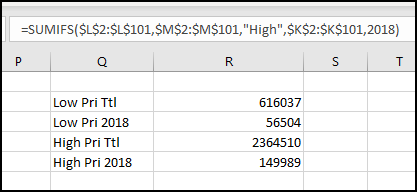
\includegraphics[width=\maxwidth{.95\linewidth}]{gfx/ch09_fig42}
		\caption{SUMIF Formula for R23}
		\label{09:fig42}
	\end{figure}
	
\end{enumerate}

\subsubsection{CountIf/CountIfS}

\[ =COUNTIF(range, criteria) \]
\[ =COUNTIFS(range1, criteria1, [range2], [criteria2], ...) \]

These two functions will count the number of cells that meet specified criteria. The difference between the two functions is that \textit{COUNTIF} can only have one criterion while \textit{COUNTIFS} can have two or more criteria. Both functions are used in the following exercise.

\begin{enumerate}
	\item This excercise uses the \fmtWorksheetName{Contacts} worksheet in the \fmtWorkbookName{Contact} workbook.
	\item Enter \fmtTyping{Low Pri Count} in cell \fmtCellLocation{Q25}.
	\item Enter \fmtTyping{Low Pri 2018} in cell \fmtCellLocation{Q26}.
	\item Enter \fmtTyping{High Pri Count} in cell \fmtCellLocation{Q27}.
	\item Enter \fmtTyping{High Pri 2018} in cell \fmtCellLocation{Q28}.
	\item Enter this formula into \fmtCellLocation{R25}: \fmtTyping{=COUNTIF(\$M\$2:\$M\$101,"Low")}. This formula counts the number of contracts with a ``Low'' priority (\fmtCellLocation{Column M}).
	\item Enter this formula into \fmtCellLocation{R26}: \fmtTyping{=COUNTIFS(\$M\$2:\$M\$101,"Low",\$K\$2:\$K\$101,2018)}. This formula counts the number of contracts with a ``Low'' priority (\fmtCellLocation{Column M}) and were signed in $ 2018 $ (\fmtCellLocation{Column K}).
	\item Enter this formula into \fmtCellLocation{R27}: \fmtTyping{=COUNTIF($M$2:$M$101,"High")}. This formula counts the number of contracts with a ``High'' priority (\fmtCellLocation{Column M}).
	\item Enter this formula into \fmtCellLocation{R28}: \fmtTyping{=COUNTIFS($M$2:$M$101,"High",$K$2:$K$101,2018)}. This formula will count the number of contracts with a ``High'' priority (\fmtCellLocation{Column M}) and were signed in $ 2018 $ (Column K).
	\item When completed, cell \fmtCellLocation{R25} should contain $ 39 $.
	\item When completed, cell \fmtCellLocation{R26} should contain $ 3 $.
	\item When completed, cell \fmtCellLocation{R27} should contain $ 30 $.
	\item When completed, cell \fmtCellLocation{R28} should contain $ 2 $.
	
	\begin{figure}[H]
		\centering
		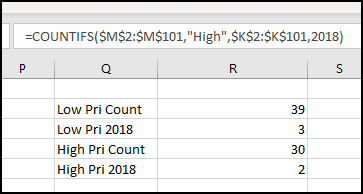
\includegraphics[width=\maxwidth{.95\linewidth}]{gfx/ch09_fig43}
		\caption{COUNTIF Formula for R28}
		\label{09:fig43}
	\end{figure}
		
\end{enumerate}

\subsubsection{Randbetween}

\[ =RANDBETWEEN(bottom, top) \]

It is common to need to generate a random number between two other numbers, like a random number between $ 1 $ and $ 10 $, and the \textit{randbetween} function makes that easy. For this exercise, assume that each of the companies in the data set need to be randomly assigned to one of  three groups for an advertising campaign. The easiest way to do that is to assign a random number between one and three to each of the companies.

\begin{enumerate}
	\item This excercise uses the \fmtWorksheetName{Contacts} worksheet in the \fmtWorkbookName{Contact} workbook.
	\item Enter \fmtTyping{Campaign} in cell \fmtCellLocation{O1}.
	\item Adjust the width of \fmtCellLocation{Column O} to properly display cell \fmtCellLocation{O1}.
	\item Enter this formula into \fmtCellLocation{O2}: \fmtTyping{=RANDBETWEEN(1,3)}. This formula will enter a random number between one and three, inclusive, into cell \fmtCellLocation{O2}.
	\item Copy cell \fmtCellLocation{O2} to \fmtCellLocation{O2:O101}. This will fill \fmtCellLocation{Column O} with random numbers between one and three.
	\item Note, in Figure \ref{09:fig44}, the numbers in cells \fmtCellLocation{O2}, \fmtCellLocation{O3}, and \fmtCellLocation{O4} were randomly assigned so student's work may display different values in those cells.
	
	\begin{figure}[H]
		\centering
		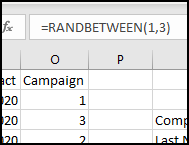
\includegraphics[width=\maxwidth{.95\linewidth}]{gfx/ch09_fig44}
		\caption{RANDBETWEEN Formula for O2}
		\label{09:fig44}
	\end{figure}
	
\end{enumerate}
	
One problem with the \textit{RandBetween} function is that new random numbers will be generated whenever any cell on the worksheet is changed. This makes it impossible to come back to the column of random numbers later and expect to find the same values. Follow these steps to correct that shortcoming.

\begin{enumerate}[resume]
	\item Select and copy \fmtCellLocation{O2:O101}.
	\item Paste Values to \fmtCellLocation{O2:O101}. Note: it is important to paste the values, not just a simple paste. Otherwise, \fmtCellLocation{O2:O101} will be filled with the \textit{RandBetween} formula rather than the value generated by that formula. Note: the values are being saved into the same cells that were used to generate the values. This is a common way used to strip a formula from a cell.
\end{enumerate}

\subsubsection{Today/Now}

\[ =TODAY() \]
\[ =NOW() \]

These two functions insert the current date into a worksheet cell. These functions must include the final parenthesis, even if they are empty. The only difference between the two functions is that \textit{today()} inserts the date while \textit{now()} inserts the date and time. Note: the format for the date and time is determined by settings on the computer. These functions are most commonly used in the header or footer in print settings.

\begin{enumerate}
	\item This excercise uses the \fmtWorksheetName{Contacts} worksheet in the \fmtWorkbookName{Contact} workbook.
	\item Insert a new column to the left of \fmtCellLocation{Column O}. The newly-inserted column becomes \fmtCellLocation{Column O}.
	\item Enter \fmtTyping{Contact\_Days} in cell \fmtCellLocation{O1}.
	\item Adjust the width of \fmtCellLocation{Column O} to properly display cell \fmtCellLocation{O1}.
	\item Enter this formula in \fmtCellLocation{O2}: \fmtTyping{=VALUE(TODAY()-N2)}. This will subtract the last contact date from today's date to determine how many days have passed since the last contact. Note: Excel will automatically format cell \fmtCellLocation{O2} as a date since \textit{today()} is in the formula. \textit{Value} makes Excel display the number of days instead of a date.
	\item Copy \fmtCellLocation{O2} to \fmtCellLocation{O3:O101}.
	
	\begin{figure}[H]
		\centering
		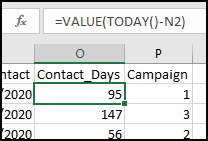
\includegraphics[width=\maxwidth{.95\linewidth}]{gfx/ch09_fig45}
		\caption{Using the Today() Function}
		\label{09:fig45}
	\end{figure}
	
\end{enumerate}

\subsubsection{Date/DateDif}

\[ =DATE(year, month, day) \]
\[ =DATEDIF (start_date, end_date, unit) \]

Excel stores dates as very large numbers and then calculates the displayed date as the number of days since January $ 1 $, $ 1900 $. For example, January $ 1 $, $ 2020 $ is stored in Excel as $ 43831 $. 

The \textit{date()} function converts a date in human-readable form to the number that Excel uses. Thus, \fmtTyping{DATE(2020,01,01)} will be converted to $ 43831 $.

The \textit{datedif()} function calculates the difference in two dates. According to the Microsoft website, ``Excel provides the \textit{DATEDIF} function in order to support older workbooks from Lotus $ 1 $-$ 2 $-$ 3 $.'' For some reason, since Excel $ 2000 $, there has been no help in the Excel system for \textit{datedif()}, but the function still works without any problems. 

The ``Unit'' option for Datedif() determines if the difference in two dates is calculated in years (\textit{Y}), months (\textit{M}), or days (\textit{D}).

\begin{enumerate}
	\item This excercise uses the \fmtWorksheetName{Contacts} worksheet in the \fmtWorkbookName{Contact} workbook.
	\item Insert a new column to the left of \fmtCellLocation{Column J}. The newly-inserted column becomes \fmtCellLocation{Column J}.
	\item Enter \fmtTyping{Age} in cell \fmtCellLocation{J1}.
	\item Enter this formula in \fmtCellLocation{J2}: \fmtTyping{=DATEDIF(I2,TODAY(),''Y'')}. This will calculate the number of years between the birthdate and today's date. 
	\item Copy \fmtCellLocation{J2} to \fmtCellLocation{J3:J101}.
	
	\begin{figure}[H]
		\centering
		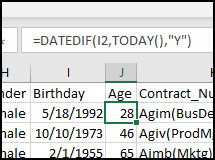
\includegraphics[width=\maxwidth{.95\linewidth}]{gfx/ch09_fig46}
		\caption{Using the Datediff() Function}
		\label{09:fig46}
	\end{figure}
	
	\item Select and copy \fmtCellLocation{J2:J101}.
	\item Paste Values to \fmtCellLocation{J2:J101}. Note: it is important to paste the values, not just a simple paste. Otherwise, \fmtCellLocation{J2:J101} will be filled with the \textit{datedif} formula rather than the value generated by that formula. Note: the values are being saved into the same cells that were used to generate the values. This is a common way used to strip a formula from a cell.
	\item Adjust the width of \fmtCellLocation{Column J} so all data is properly displayed.
\end{enumerate}

\subsubsection{AND/OR}

\[ =AND(logical1, [logical2], ...) \]
\[ =OR(logical1, [logical2], ...) \]

These two related functions test different logical conditions and return either \textit{TRUE} or \textit{FALSE} depending on the outcome of the test. 

\begin{enumerate}
	\item This excercise uses the \fmtWorksheetName{Contacts} worksheet in the \fmtWorkbookName{Contact} workbook.
	\item Insert a new column to the left of \fmtCellLocation{Column K}. The newly-inserted column becomes \fmtCellLocation{Column K}.
	\item Enter \fmtTyping{Sales} in cell \fmtCellLocation{K1}.
	\item Enter this formula in \fmtCellLocation{K2}: \fmtTyping{=AND(G2 = "Sales", J2 < 40)}. This will output \textit{TRUE} if \fmtCellLocation{G2} contains ``Sales'' and \fmtCellLocation{J2} is less than $ 40 $. 
	\item Copy \fmtCellLocation{K2} to \fmtCellLocation{K3:K101}.
	
	\begin{figure}[H]
		\centering
		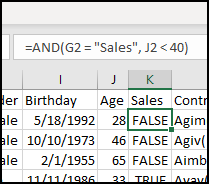
\includegraphics[width=\maxwidth{.95\linewidth}]{gfx/ch09_fig47}
		\caption{Using the AND Function}
		\label{09:fig47}
	\end{figure}
	
	\item Adjust the width of \fmtCellLocation{Column K} so all data is properly displayed.

	\item Normally, \textit{AND} and \textit{OR} functions are combined with an \textit{IF} function to make the result more readable.
	\item Change the formula in \fmtCellLocation{K2} to this: \fmtTyping{=IF(AND(G2 = "Sales", J2 < 40),"Yes","")}. This will print \textit{Yes} for lines where the Role (\fmtCellLocation{Column F})is \textit{Sales} and Age (\fmtCellLocation{Column J}) is less than $ 40 $ but print nothing otherwise. 
	\item Copy \fmtCellLocation{K2} to \fmtCellLocation{K3:K101}. Now most cells in \fmtCellLocation{Column K} will be blank but a few will contain \textit{Yes}.
\end{enumerate}

\subsubsection{NOT}

\[ =NOT(logical) \]

This function will test different a logical condition and return either \textit{TRUE} or \textit{FALSE} depending on the outcome of the test.

\begin{enumerate}
	\item This excercise uses the \fmtWorksheetName{Contacts} worksheet in the \fmtWorkbookName{Contact} workbook.
	\item Insert a new column to the left of \fmtCellLocation{Column E}. The newly-inserted column becomes \fmtCellLocation{Column E}.
	\item Enter \fmtTyping{Common} in cell \fmtCellLocation{E1}.
	\item Enter this formula in \fmtCellLocation{E2}: \fmtTyping{=NOT(D6="Dr")}. This will output \textit{TRUE} if \fmtCellLocation{E2} contains anything other than \textit{Dr}. 
	\item Copy \fmtCellLocation{E2} to \fmtCellLocation{E3:E101}.
	
	\begin{figure}[H]
		\centering
		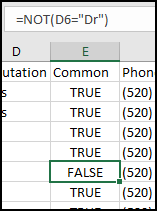
\includegraphics[width=\maxwidth{.95\linewidth}]{gfx/ch09_fig48}
		\caption{Using the NOT Function}
		\label{09:fig48}
	\end{figure}
	
	\item To make the search a bit more robust, change \fmtCellLocation{E2} to: \fmtTyping{=AND(NOT(D2="Dr"),NOT(D2="Rev"))}. This formula uses AND to look for Salutations (\fmtCellLocation{Column D}) that are not \textit{Dr} and not \textit{Rev}.
	\item As one final improvement in the formula, change \fmtCellLocation{E2} to this: \fmtTyping{=IF(AND(NOT(D2="Dr"),NOT(D2="Rev")),"Yes","")}. This will print \textit{Yes} for lines where the Salutation (\fmtCellLocation{Column D}) is anything other than ``Dr'' and ``Rev'' but print nothing otherwise.	
	\item Copy \fmtCellLocation{E2} to \fmtCellLocation{E3:E101}.
	\item Adjust the width of \fmtCellLocation{Column E} so all data is properly displayed.
\end{enumerate}

%\subsection{Examples}
%
%Here is an example that combine both text and number functions.
%
%	\item Extract information for the oldest person in the list
%	\item See \url{https://exceljet.net/formula/get-information-corresponding-to-max-value}

\begin{center}
	\begin{tkwbox}{Key Take-Aways}
		\textbf{x}
		\\
		\begin{itemize}
			\setlength{\itemsep}{0pt}
			\setlength{\parskip}{0pt}
			\setlength{\parsep}{0pt}
			
			\item Excel includes hundreds of functions for both text and numbers, but some are more generally useful than others.  
			\item Excel's most useful text functions include To Columns, Trim, Concatenate, Upper/Lower/Proper, Left/Right/Mid, VLookup, and Index Match.
			\item Excel's most useful number functions include Sum, Average, Min/Max, Round, If, SumIf, CountIf, RandBetween, Today/Now, Date/DateDif, AND/OR, and NOT.
			
		\end{itemize}
	\end{tkwbox}
\end{center}

%\section{Get \& Transform}
%
%\begin{center}
%	\begin{objbox}{Learning Objectives}
%		\begin{itemize}
%			\setlength{\itemsep}{0pt}
%			\setlength{\parskip}{0pt}
%			\setlength{\parsep}{0pt}
%			
%			\item one
%			
%		\end{itemize}
%	\end{objbox}
%\end{center}
%
%Excel can load data from numerous sources including web-based content, .CSV files, database links, Microsoft Azure, and Access databases, among many others. That data often needs to be ``shaped'' while it is imported. The shaping process could complete tasks on columns like renaming, moving, or eliminating them altogether. Also, missing data can be addressed in several different ways. This entire process is handled by Excel's Power Query tool. While Power Query is quite complex and many of its features are beyond the scope of this book, it can be useful for even simple data import projects.
%
%A Power Query connects Excel to a data source. Queries can be as simple as importing data from a .CSV file, which was completed elsewhere in this book; but it can also be as complex as creating an SQL link to some commercial database. The data can be transformed and saved to a table. The query is also saved and can be rerun to get updated data from the database. Queries can also be shared so people working on the same project can extract the data as needed.
%
%\subsubsection{Starting Power Query}
%
%\begin{itemize}
%	\item For Excel \fmtExcelOld{2016}
%
%	\begin{enumerate}
%		\item Click \fmtRibbonButton{Data $ \Rightarrow $ Get \& Transform $ \Rightarrow $ New Query $ \Rightarrow $ From File $ \Rightarrow $ From CSV}.
%		
%		\begin{figure}[H]
%			\centering
%			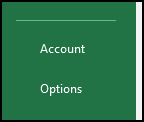
\includegraphics[width=\maxwidth{.95\linewidth}]{gfx/ch09_fig50}
%			\caption{Starting Power Query in Excel 2016}
%			\label{09:fig50}
%		\end{figure}
%		
%		\item Navigate to \fmtWorkbookName{CH9-Query.CSV} and click \fmtPopupButton{Open}.	
%	\end{enumerate}
%
%	\item For Excel \fmtExcelNew{365}
%
%	\begin{enumerate}
%		\item Click \fmtRibbonButton{Data $ \Rightarrow $ Get \& Transform Data $ \Rightarrow $ Get Data $ \Rightarrow $ From File $ \Rightarrow $ From Text/CSV}.
%		
%		\begin{figure}[H]
%			\centering
%			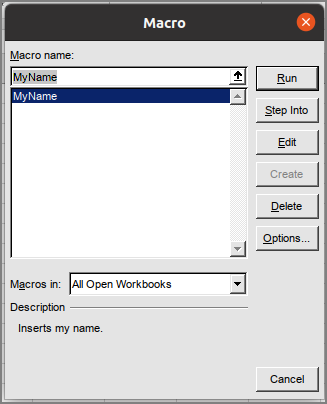
\includegraphics[width=\maxwidth{.95\linewidth}]{gfx/ch09_fig51}
%			\caption{Starting Power Query in Excel 365}
%			\label{09:fig51}
%		\end{figure}
%		
%		\item Navigate to \fmtWorkbookName{CH9-Query.CSV} and click \fmtPopupButton{Import}.	
%	\end{enumerate}
%
%\end{itemize}
%
%\subsubsection{Using Power Query}
%
%\begin{enumerate}
%	\item Following either procedure above will open the Data Import window.
%
%	\begin{figure}[H]
%		\centering
%		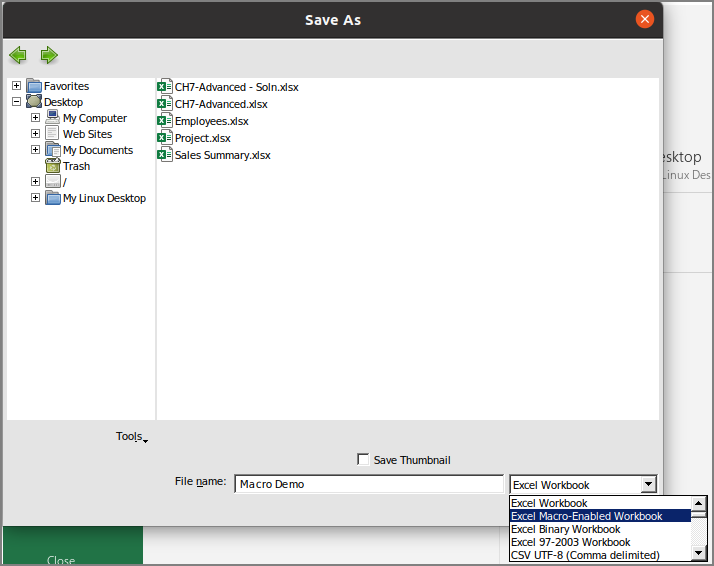
\includegraphics[width=\maxwidth{.95\linewidth}]{gfx/ch09_fig52}
%		\caption{Data Import Window}
%		\label{09:fig52}
%	\end{figure}
%	
%	\item From  this point, the Power Query process is the same for both Excel $ 2016 $ and Excel $ 365 $. 
%	\item Click \fmtPopupButton{Transform Data}. Note: be sure to click the \fmtPopupButton{Transform Data} button rather than the \fmtPopupButton{Load} button.
%	\item The Power Query window has a ribbon bar with many different tools, a large preview area, and the query's \textit{Applied Steps} section on the right. As various tools are selected and applied to the data the steps will increase to show the process used.
%	\item Click the down arrow for the \fmtCellLocation{length} column and sort the column ascending.
%
%	\begin{figure}[H]
%		\centering
%		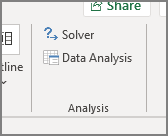
\includegraphics[width=\maxwidth{.95\linewidth}]{gfx/ch09_fig53}
%		\caption{Sorting a Column}
%		\label{09:fig53}
%	\end{figure}
%
%	\item Notice that the top three rows have \textit{null} values. That means that the original .CSV file was missing length data for those rows. Missing data often fouls statistical analysis so these three rows should be deleted. To do that, click \fmtRibbonButton{Reduce Rows $ \Rightarrow $ Remove Rows}. 
%
%
%
%
%
%
%
%
%
%
%
%\end{enumerate}
%
%Lorem ipsum dolor sit amet, consectetur adipiscing elit. Nulla id congue orci. Nullam aliquam nulla orci, quis pulvinar lectus sodales a. Donec vel nunc sit amet leo faucibus volutpat id a arcu. Proin facilisis feugiat libero, a sodales enim ultrices quis. Morbi vitae lorem sagittis, porta lacus sit amet, gravida urna. Nulla pellentesque tempor turpis, non convallis turpis commodo a. Nunc auctor sed erat ac elementum. 
%
%\begin{center}
%	\begin{tkwbox}{Key Take-Aways}
%		\textbf{x}
%		\\
%		\begin{itemize}
%			\setlength{\itemsep}{0pt}
%			\setlength{\parskip}{0pt}
%			\setlength{\parsep}{0pt}
%			
%			\item one
%			
%		\end{itemize}
%	\end{tkwbox}
%\end{center}

\section{Statistics}

\begin{center}
	\begin{objbox}{Learning Objectives}
		\begin{itemize}
			\setlength{\itemsep}{0pt}
			\setlength{\parskip}{0pt}
			\setlength{\parsep}{0pt}
			
			\item The Excel Data Analysis pack includes $ 19 $ advanced statistics functions.
			\item Correlation, Descriptives, and Histogram are easy to understand and demonstrate the power of the Data Analysis pack.
			
		\end{itemize}
	\end{objbox}
\end{center}

Excel includes an \textit{Analysis Toolpak} that contains $ 19 $ advanced statistics and engineering functions, but it is considered an Add-in and must be activated before it can be used. Most Excel users will never need these types of statistics analysis tools, but they are available if needed.

\begin{enumerate}
	\item Click \fmtRibbonTab{File} to open the backstage view.
	\item In the backstage view, click \fmtRibbonButton{Options} at the bottom of the left-hand menu.
	
\end{enumerate}

\begin{figure}[H]
	\centering
	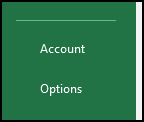
\includegraphics[width=\maxwidth{.95\linewidth}]{gfx/ch09_fig50}
	\caption{The Options Button in the Backstage View}
	\label{09:fig50}
\end{figure}

\begin{enumerate}[resume]	
	
	\item Click \fmtPopupButton{Add-ins} in the left-hand menu of the \fmtPopupBox{Excel Options} pop-up box.
	\item Select \fmtPopupBox{Excel Add-ins} in the drop-down menu at the bottom of the \fmtPopupBox{Add-ins} tab.
	\item Click \fmtPopupButton{Go}.
	
\end{enumerate}

\begin{figure}[H]
	\centering
	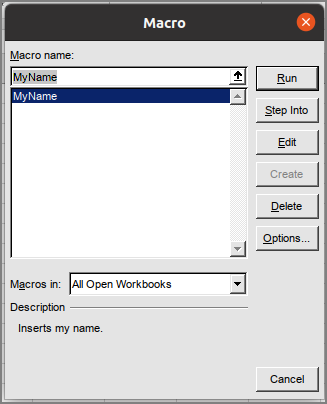
\includegraphics[width=\maxwidth{.95\linewidth}]{gfx/ch09_fig51}
	\caption{The Add-ins Manager}
	\label{09:fig51}
\end{figure}

\begin{enumerate}[resume]	
	
	\item Click the checkbox beside \fmtPopupBox{Analysis Toolpak Add-in} in the \fmtPopupBox{Add-ins} pop-up box.
	
\end{enumerate}

\begin{figure}[H]
	\centering
	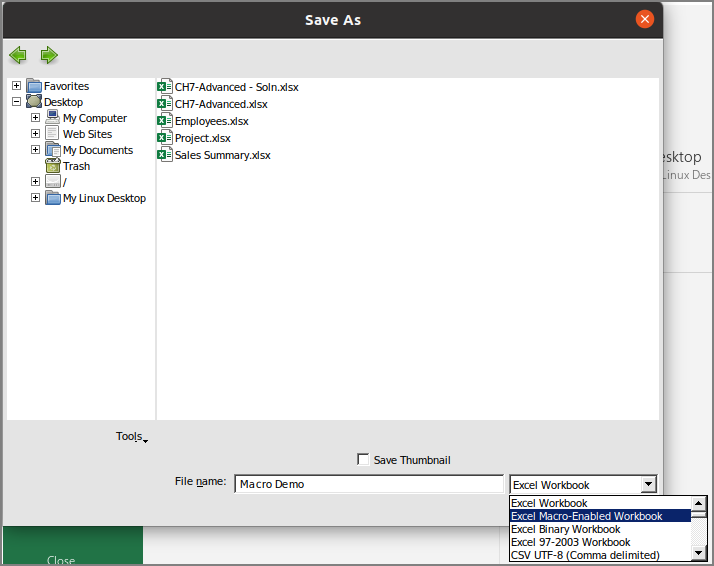
\includegraphics[width=\maxwidth{.95\linewidth}]{gfx/ch09_fig52}
	\caption{Activating The Analysis Toolpak Add-In}
	\label{09:fig52}
\end{figure}

\begin{enumerate}[resume]	
	\item Click \fmtPopupButton{OK}.
\end{enumerate}

There is a new button at Click \fmtRibbonButton{Data $ \Rightarrow $ Analysis $ \Rightarrow $ Data Analysis}.

\begin{figure}[H]
	\centering
	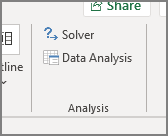
\includegraphics[width=\maxwidth{.95\linewidth}]{gfx/ch09_fig53}
	\caption{The Data Analysis Button}
	\label{09:fig53}
\end{figure}

\begin{enumerate}[resume]	
	\item Open workbook \fmtWorkbookName{CH9-Stats.xlsx}
	\item This workbook has only one worksheet, \fmtWorksheetName{Cafe}.
\end{enumerate}

The Cafe worksheet contains $ 100 $ results of a survey of customers in a small cafe. Note: this is dummy data created for this book.

\subsubsection{Correlation}

A fundamental statistical calculation is the correlation between two variables. A correlation is a number between $ -1.0 $ and $ +1.0 $, where $ 0.0 $ means there is no correlation between the two variables and either $ +1.0 $ or $ -1.0 $ means there is a perfect correlation. A positive correlation means that as one variable increases the other also increases. For example, as people age they tend to weigh more so a positive correlation would be expected between age and weight. A negative correlation, on the other hand, means that as one variable increases the other decreases. For example, as people age they tend to run slower so a negative correlation would be expected between age and running speed. For the Cafe data, it would be reasonable to wonder if there is some sort of relationship between the length of the meal and the bill. It would seem that longer meals should correlate to higher bills, so a positive correlation of more than $ +0.5 $ would be important for a researcher to know.

\begin{enumerate}[resume]
	\item Click \fmtRibbonButton{Data $ \Rightarrow $ Analysis $ \Rightarrow $ Data Analysis}.
	\item From the popup box, select \fmtPopupBox{Correlation} and click \fmtPopupButton{OK}.
\end{enumerate}

\begin{figure}[H]
	\centering
	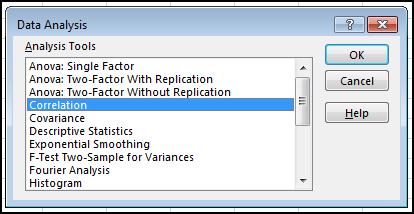
\includegraphics[width=\maxwidth{.95\linewidth}]{gfx/ch09_fig54}
	\caption{Data Analysis Selection Box}
	\label{09:fig54}
\end{figure}

\begin{enumerate}[resume]
	\item The \fmtPopupBox{Correlation Parameters} box pops up.
\end{enumerate}

\begin{figure}[H]
	\centering
	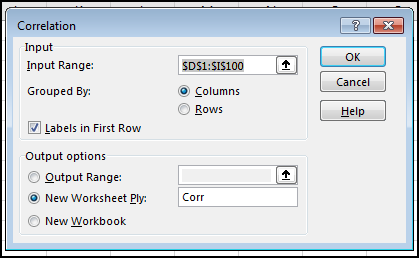
\includegraphics[width=\maxwidth{.95\linewidth}]{gfx/ch09_fig55}
	\caption{Correlation Parameters}
	\label{09:fig55}
\end{figure}

\begin{enumerate}[resume]
	\item Input Range: \fmtTyping{\$D\$1:\$I\$100}
	\item Grouped By: Columns
	\item Labels in First Row: Checked
	\item Output: New Worksheet Named \fmtTyping{Corr}
	\item Click \fmtPopupButton{OK}.
	\item Excel creates a new worksheet named Corr that contains a correlation table that displays the correlations between the six variables contained in the selected range. Notice that the correlation between \textit{Length} and \textit{Bill} is $ 0.611327 $, which is strong. However, also note that the correlation between \textit{PtySize} (the number in the group) and \textit{Bill} is $ 0.866466 $, which is much stronger. It would stand to reason that a larger group of diners would generate a higher bill.
\end{enumerate}

\begin{figure}[H]
	\centering
	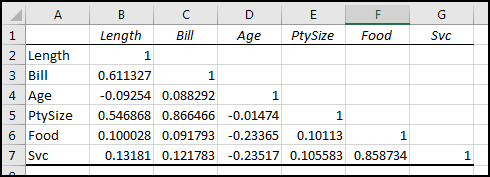
\includegraphics[width=\maxwidth{.95\linewidth}]{gfx/ch09_fig56}
	\caption{Correlation Table}
	\label{09:fig56}
\end{figure}

\subsubsection{Descriptives}

Descriptive statistics summarize a variable with multiple useful calculations. Follow these steps to generate descriptives for \textit{Age}.

\begin{enumerate}[resume]
	\item Click \fmtRibbonButton{Data $ \Rightarrow $ Analysis $ \Rightarrow $ Data Analysis}.
	\item From the popup box, select \fmtPopupBox{Descriptive Statistics} and click \fmtPopupButton{OK}.
	\item The \fmtPopupBox{Descriptive Statistics Parameters} box pops up.
\end{enumerate}

\begin{figure}[H]
	\centering
	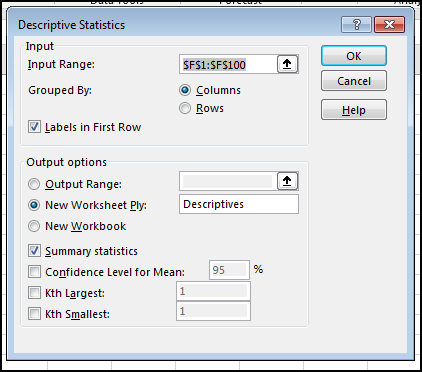
\includegraphics[width=\maxwidth{.95\linewidth}]{gfx/ch09_fig60}
	\caption{Descriptive Statistics Parameters}
	\label{09:fig60}
\end{figure}

\begin{enumerate}[resume]
	\item Input Range: \fmtTyping{\$F\$1:\$F\$100}
	\item Grouped By: Columns
	\item Labels in First Row: Checked
	\item Output: New Worksheet Named \fmtTyping{Descriptives}
	\item Summary Statistics: Checked
	\item Click \fmtPopupButton{OK}.
	\item Excel creates a new worksheet named Descriptives that contains a table that displays various descriptive statistics for \textit{Age}. For example, the mean age is $ 41.47475 $.
\end{enumerate}

\begin{figure}[H]
	\centering
	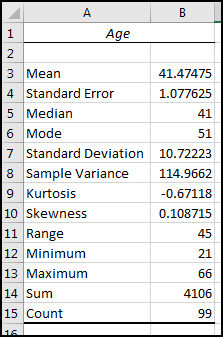
\includegraphics[width=\maxwidth{.95\linewidth}]{gfx/ch09_fig61}
	\caption{Descriptive Statitics}
	\label{09:fig61}
\end{figure}

\subsubsection{Histogram}

A histogram is a graphic representation of a numeric variable. For a histogram, the values are placed in ``bins'' and the number in each bin is counted and graphed. 

\begin{enumerate}[resume]
	\item Click \fmtRibbonButton{Data $ \Rightarrow $ Analysis $ \Rightarrow $ Data Analysis}.
	\item From the popup box, select \fmtPopupBox{Histogram} and click \fmtPopupButton{OK}.
	\item The \fmtPopupBox{Histogram Parameters} box pops up.
\end{enumerate}

\begin{figure}[H]
	\centering
	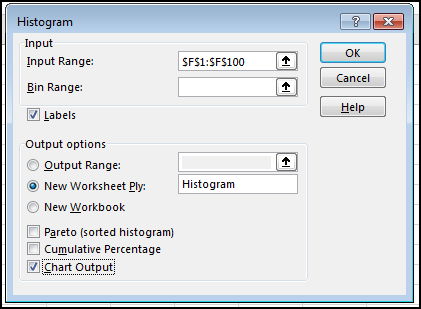
\includegraphics[width=\maxwidth{.95\linewidth}]{gfx/ch09_fig62}
	\caption{Histogram Parameters}
	\label{09:fig62}
\end{figure}

\begin{enumerate}[resume]
	\item Input Range: \fmtTyping{\$F\$1:\$F\$100}
	\item Bin Range: leave blank
	\item Labels: Checked
	\item Output: New Worksheet Named \fmtTyping{Histogram}
	\item Chart Output: Checked
	\item Click \fmtPopupButton{OK}.
	\item Excel creates a new worksheet named Histogram that contains a table that displays the counts for each age ``bin.'' For example, $ 15 $ people were between the ages of $ 36 $ and $ 40 $. Also, the histogram graph is displayed for a quick view of how the age data is distributed.
\end{enumerate}

\begin{figure}[H]
	\centering
	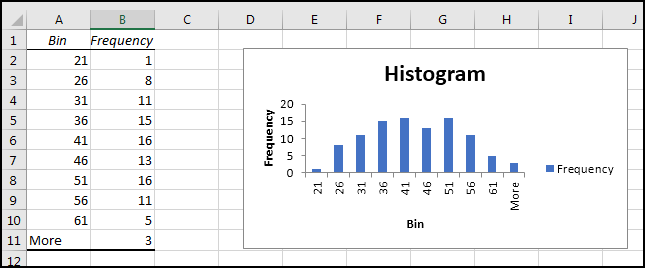
\includegraphics[width=\maxwidth{.95\linewidth}]{gfx/ch09_fig63}
	\caption{Histogram of Age}
	\label{09:fig63}
\end{figure}

\begin{center}
	\begin{tkwbox}{Key Take-Aways}
		\textbf{x}
		\\
		\begin{itemize}
			\setlength{\itemsep}{0pt}
			\setlength{\parskip}{0pt}
			\setlength{\parsep}{0pt}
			
			\item A correlation numerically describes the relationship between two variables.
			\item Descriptives create numerous statistics for a variable.
			\item A histogram graphically represents the distribution for a numeric variable.
			
		\end{itemize}
	\end{tkwbox}
\end{center}

\section{Macros}

\begin{center}
	\begin{objbox}{Learning Objectives}
		\begin{itemize}
			\setlength{\itemsep}{0pt}
			\setlength{\parskip}{0pt}
			\setlength{\parsep}{0pt}
			
			\item Automate simple tasks with a macro.
			
		\end{itemize}
	\end{objbox}
\end{center}

\fmtRibbonButton{View $ \Rightarrow $ Macros $ \Rightarrow $ Macros} allows users to automate repetitive tasks. The top part of the button will open the \fmtPopupBox{View Macros} dialog box and the bottom half reveals options for macros. 

\begin{enumerate}
	\item Open a new blank workbook. (\textit{Note}: the macro is placed in a new workbook so it does not accidentally interfere with the exercises in any other workbook.)
	\item Click \fmtCellLocation{A1} to select that cell.
	\item Click \fmtRibbonButton{View $ \Rightarrow $ Macros $ \Rightarrow $ Macros} (be sure to click the small arrow at the bottom of the \fmtRibbonButton{Macros} button).
	\item Select \fmtPopupButton{Use Relative References}.
	\item In the same popup, select \fmtPopupButton{Record Macro}.
	\item Name the macro \fmtTyping{MyName}.
	\item Click in the \fmtPopupBox{Shortcut Key} box and type \fmtKeystroke{Q}.
	\item Store the macro in this workbook.
	\item Enter this description: \fmtTyping{Inserts my name}.
\end{enumerate}

\begin{figure}[H]
	\centering
	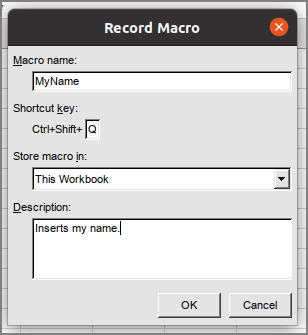
\includegraphics[width=\maxwidth{.95\linewidth}]{gfx/ch09_fig65}
	\caption{The Record Macro Settings Box}
	\label{09:fig65}
\end{figure}

\begin{enumerate}[resume]	
	\item Click \fmtPopupButton{OK}.
	\item Type your first and last name and press \fmtKeystroke{Enter}.
	\item Click \fmtRibbonButton{View $ \Rightarrow $ Macros $ \Rightarrow $ Macros} (be sure to click the small arrow at the bottom of the \fmtRibbonButton{Macros} button).
	\item Select \fmtPopupButton{Stop Recording}.
\end{enumerate}

Select another cell on the worksheet and press \fmtKeystroke{Ctrl} $ + $ \fmtKeystroke{Shift} $ + $ \fmtKeystroke{Q}. Remember that relative references were activated for the macro, otherwise the name would have always been created in cell \fmtCellLocation{A1} (the original cell) instead of the current cell.

\begin{enumerate}
	\item Click \fmtRibbonButton{View $ \Rightarrow $ Macros $ \Rightarrow $ Macros} (be sure to click the top of the \fmtRibbonButton{Macros} button).
	\item This opens the Macro manager dialog where macros can be edited, deleted, or have various options set.
\end{enumerate}

\begin{figure}[H]
	\centering
	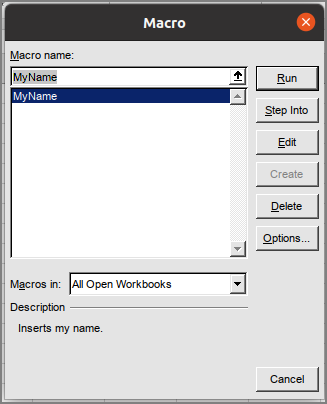
\includegraphics[width=\maxwidth{.95\linewidth}]{gfx/ch09_fig66}
	\caption{The Macro Manager Box}
	\label{09:fig66}
\end{figure}

\begin{enumerate}[resume]	
	\item Click \fmtPopupButton{Cancel} to close the Macro manager.
\end{enumerate}

Remember that all workbooks containing macros must be saved using the ``macro-enabled'' option (that creates a file extension of \textit{.xlsm}). Figure \ref{09:fig67} shows a drop-down menu at the bottom right corner of the \fmtPopupBox{Save-As} screen where \fmtPopupButton{Excel Macro-Enabled Workbook} must be selected. 

\begin{figure}[H]
	\centering
	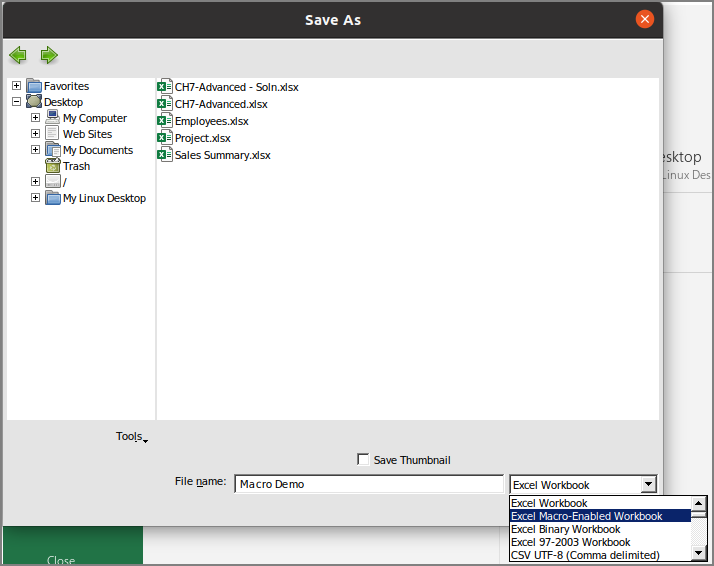
\includegraphics[width=\maxwidth{.95\linewidth}]{gfx/ch09_fig67}
	\caption{Saving a Workbook With a Macro}
	\label{09:fig67}
\end{figure}

Since this macro will not be reused in the future, close the workbook without saving.

\begin{center}
	\begin{tkwbox}{Key Take-Aways}
		\textbf{Using Excel Macros}
		\\
		\begin{itemize}
			\setlength{\itemsep}{0pt}
			\setlength{\parskip}{0pt}
			\setlength{\parsep}{0pt}
			
			\item Macros automate simple tasks to save time in data entry.
			\item Workbooks containing macros must be saved with the ``Macro-Enabled'' setting.
			
		\end{itemize}
	\end{tkwbox}
\end{center}

\section{Excel Preferences}

\begin{center}
	\begin{objbox}{Learning Objectives}
		\begin{itemize}
			\setlength{\itemsep}{0pt}
			\setlength{\parskip}{0pt}
			\setlength{\parsep}{0pt}
			
			\item Explore and optionally change Excel preferences.
			
		\end{itemize}
	\end{objbox}
\end{center}

Like all Microsoft Office products, Excel has scores of preferences and this section lists those that are most commonly changed by users.

To find the preferences, click \fmtRibbonButton{File $ \Rightarrow $ Options}.

\begin{figure}[H]
	\centering
	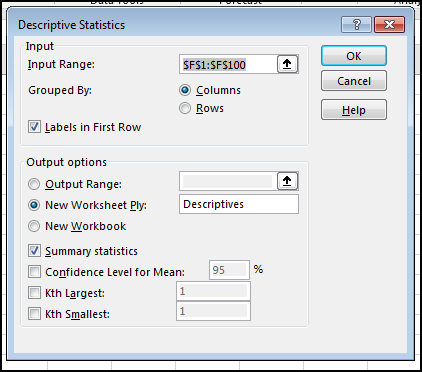
\includegraphics[width=\maxwidth{.95\linewidth}]{gfx/ch09_fig60}
	\caption{The Backstage Options Button}
	\label{09:fig60}
\end{figure}
 
The Options area is divided into $ 11 $ different tabs and each tab includes settings for many preferences. Here is a brief overview of the different option tabs.

\begin{table}[H]
	\rowcolors{1}{}{tablerow} % zebra striping background
	{\small
		%\fontsize{8}{10} \selectfont %Replace small for special font size
		\begin{longtable}{L{1.00in}L{3.00in}} %Left-aligned, Max width: 4.25in
			\textbf{Category} & \textbf{Settings} \endhead
			\hline
			General & These are the commonly-modified settings, such as the user interface, customer name, and Start screen.\\
			Formulas & Settings to control calculations, error-checking, and formulas.\\
			Proofing & Options for spell-check and auto-correct.\\
			Save & Settings that govern saving, autorecovery, and web server options.\\
			Language & Chose the primary and other languages used for editing, tooltips, and help.\\
			Ease of Access & Settings that concern accessibility, including an accessibility checker and various settings for sounds and font.\\
			Advanced & Numerours settings that are not often changed, divided into five areas.\\
			Customize Ribbon & Add and remove items from the ribbon, also rearrange or rename the ribbon tabs and groups.\\
			Quick Access Toolbar & Add and remove items from the Quick Access Toolbar, rearrange the toolbar, and specify its location.\\
			Add-ins & Activate or remove various add-ins.\\
			Trust Center & Manage certificates and other Excel security features.\\
			\rowcolor{captionwhite}
			\caption{Summary of Excel Options}
			\label{09:tab03}
		\end{longtable}
	} % End small
\end{table}

It is not the intent of this book to describe every possible preference, but following is a list of those that users commonly modify.

\subsection{General}

\begin{description}
	\item[Enable Live Preview] When changing visual items, like fonts or colors, this previews the change live in the current sheet. This can get annoying so some users turn it off.
	\item[Screen Tip style] Screen tips are the pop-up boxes with brief help for the various buttons on the ribbon. Some users find these distracting and the can be turned off with this setting.
	\item[Use this as the default font] Use this to change the default font used in new workbooks. Also, the default font size can be set if a larger size is needed.
	\item[Include this many sheets] New workbooks include three blank worksheets by default, but that number can be changed here. Often, one worksheet is enough for new workbooks and then other worksheets can added as needed.
	\item[User name] This is the author's name that is saved with the workbook.
	\item[Show the Start screen when this application starts] Uncheck this box to turn off the start screen.
	\item[Collapse the ribbon automatically] Checking this box will automatically collapse the ribbon into a menu in order to save space on the screen. The ribbon will drop down when any of the menu items are clicked. It is also easy to pin the ribbon open while working.
\end{description}

\subsection{Formulas}

\begin{description}
	\item[Reset Ignored Errors] Sometimes users have Excel ignore errors as they are developing a worksheet. This button will reset the ignored errors so all errors are again displayed.
\end{description}

\subsection{Proofing}

This tab includes the various settings for spell-check, like ignore uppercase words. It also includes the Autocorrect options. Normally, the default settings for these items is adequate but that can be changed at this tab.

\subsection{Save}

\begin{description}
	\item[Save AutoRecover information every] Set how often Excel autosaves a workbook. The default is $ 10 $ minutes, but that can be decreased if desired.
	\item[Default local file location] This is the default location for files on initial save or a ``Save As'' operation.
\end{description}

\subsection{Language}

Excel uses the Windows system language and that is normally acceptable. However, this tab makes it possible to change the default Office language for both viewing and editing.

\subsection{Ease of Access}

This tab makes a number of accessibility options available. 

\subsection{Advanced}
	
	\begin{description}
		\item[After pressing Enter, move selection] By default, Excel moves the selector (active cell) down when the enter key is pressed, but some users prefer the selector to move right and that can be set here.
		\item[Show this number of Recent Workbooks] When Excel opens, it displays the file names for recently-opened workbooks. Use this preference to set the number of recent workbooks to display. The default (and maximum number) is $ 50 $.
		\item[Ruler units] Most Americans are comfortable using inches on the ruler, but Excel can also use metric units. The unit used is set with this preference.
		\item[At startup, open all files in] Specify a folder on the hard drive and any Excel files in that folder will be automatically opened when Excel starts. This is a great timesaver while working on a project for several weeks where the same Excel files need to be opened.
	\end{description}
	
\subsection{Customize Ribbon}

The ribbon is highly customizable from this tab. Users can add/remove items from the ribbon, change the order of the items on the ribbon, create new groups, rename items, and generally whatever they want to do to make the ribbon work best for themselves. Customizations can even be exported in a file that can be imported on another computer so users can make Excel on all of the computers they use look the same.

In addition to the customizations on this tab, the General Tab includes an option to collapse the ribbon automatically.

\subsection{Quick Access Toolbar}

The Quick Access Toolbar is one of the most useful Excel feature. Users can add links to their most often used Excel functions so they are easily available without clicking on any ribbon links. The Quick Access Toolbar is set up with the links the user wants. Optionally, the Quick Access Toolbar can be moved to under the ribbon.

\subsection{Add-ins}

Any add-ins present in Excel can be activated/deactivated from this tab.

\subsection{Trust Center}

Users can check security certificates or other security settings on this tab.

\begin{center}
	\begin{tkwbox}{Key Take-Aways}
		\textbf{Preferences}
		\\
		\begin{itemize}
			\setlength{\itemsep}{0pt}
			\setlength{\parskip}{0pt}
			\setlength{\parsep}{0pt}
			
			\item Excel includes scores of options that users can change according to their individual preferences.
			
		\end{itemize}
	\end{tkwbox}
\end{center}

\section{Chapter Practice}

\subsection{Cars Analysis}

This exercise uses data on $ 392 $ car models that was collected by David Donoho and Ernesto Ramos for the $ 1982 $ \textit{Exposition of Statistical Graphics Technology} hosted by the \textit{Committee on Statistical Graphics of the American Statistical Association (ASA)}. The dataset is commonly-used in statistics classes and can be found at several online locations, including \url{https://github.com/sandialabs/slycat-data}.

\begin{enumerate}
	\item Start Excel and open a blank workbook.
	\item Save the workbook as \fmtWorkbookName{PR9-Cars}.
	\item \fmtExcelNew{365} Load the data.
	
	\begin{enumerate}
		\item Click \fmtRibbonButton{Data $ \Rightarrow $ Get \& Transform Data $ \Rightarrow $ From Text/CSV}.
		\item Navigate to \fmtWorkbookName{PR9-Data.csv}.
		\item Click the file name and then \fmtPopupButton{Import}.
		\item Excel correctly identifies the data fields in the file, so click \fmtPopupButton{Load} to import the data into a table in a new worksheet.	
	\end{enumerate}		

	\item \fmtExcelOld{2016} Load the data.
		
	\begin{enumerate}		
		\item \fmtRibbonButton{Get External Data} in the \fmtRibbonTab{Data} tab of the ribbon.
		\item Click \fmtPopupButton{From Text}. 
		\item Navigate to \fmtWorkbookName{PR9-Data.csv}.
		\item Click the file name and then \fmtPopupButton{Import}.
		\item Import the data file into a new worksheet.
		\begin{enumerate}
			\item The data in the CSV file has headers.
			\item The data uses a comma delimiter.
			\item Import the data into a new worksheet.
		\end{enumerate}
	\end{enumerate}
		
	\item Rename \fmtWorksheetName{Sheet2} to \fmtWorksheetName{Cars}.
	\item Delete \fmtWorksheetName{Sheet1}.
	\item Click A1 to activate the table.
	\item Enter \fmtTyping{Cars} in \fmtRibbonButton{Table Design $ \Rightarrow $ Properties $ \Rightarrow $ Table Name}.
\end{enumerate}

\begin{enumerate}[resume]

	\item Even though the data loads properly, there are a few adjustments that need to be made. First, the \fmtCellLocation{Origin} column only lists three different locations by number, but these should be changed to their text equivalent for easier analysis.
	
	\begin{enumerate}
		\item Click the down-arrow on the right side of the \textit{Origin} column header for \fmtCellLocation{Column I}.
		\item Uncheck all items except \fmtPopupButton{$ 1 $}.

		\begin{figure}[H]
			\centering
			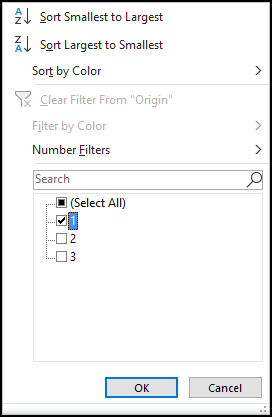
\includegraphics[width=\maxwidth{.95\linewidth}]{gfx/ch09_fig70}
			\caption{Filtering for Location $ 1 $}
			\label{09:fig70}
		\end{figure}

		\item All rows that do not contain a $ 1 $ for \textit{Origin} are hidden. 
		\item Enter \fmtTyping{American} in \fmtCellLocation{I3} (the cell at the top of the column after rows have been hidden).
		\item Copy/paste \fmtCellLocation{I3} to all other visible cells in \fmtCellLocation{Column I}.	Note: using the autofill handle makes this task easier.
		
		\item Click the filter symbol on the right side of the \textit{Origin} column header for \fmtCellLocation{Column I}.
		\item Uncheck all items except \fmtPopupButton{$ 2 $}.
		\item All rows that do not contain a $ 2 $ for \textit{Origin} are hidden. 
		\item Enter \fmtTyping{European} in \fmtCellLocation{I2} (the cell at the top of the column after rows have been hidden).
		\item Copy/paste \fmtCellLocation{I2} to all other visible cells in \fmtCellLocation{Column I}.	Note: using the autofill handle makes this task easier.

		\item Click the filter symbol on the right side of the \textit{Origin} column header for \fmtCellLocation{Column I}.
		\item Uncheck all items except \fmtPopupButton{$ 3 $}.
		\item All rows that do not contain a $ 3 $ for \textit{Origin} are hidden. 
		\item Enter \fmtTyping{Japanese} in \fmtCellLocation{I4} (the cell at the top of the column after rows have been hidden).
		\item Copy/paste \fmtCellLocation{I4} to all other visible cells in \fmtCellLocation{Column I}.	Note: using the autofill handle makes this task easier.
		
		\item Click the filter symbol on the right side of the \textit{Origin} column header for \fmtCellLocation{Column I}.
		\item Check \fmtPopupButton{(Select All)} to reveal all rows in the data set.

	\end{enumerate}

	\item Next, data in the \fmtCellLocation{Model} column needs to be split out so the automobile make and model are separated.
	
	\begin{enumerate}
		\item Insert a column to the left of \fmtCellLocation{Column B}. The new column becomes \fmtCellLocation{Column B} with a header of \textit{Column1}.
		\item Enter this formula in \fmtCellLocation{B2}: \fmtTyping{=PROPER(LEFT(A2,FIND(" ",A2)-1))}. If Excel does not paste that formula to the bottom of the table, then copy/paste it to \fmtCellLocation{B3:B393}. Excel extracts the make of the car, which is the first word in \fmtCellLocation{Column A}.
		\item Insert a column to the left of \fmtCellLocation{Column C}. The new column becomes \fmtCellLocation{Column C} with a header of \textit{Column2}.
		\item Copy \fmtCellLocation{B2:B393}.
		\item Paste Values to \fmtCellLocation{C2}. Note: it is important to paste the values, not just a simple paste. Otherwise, \fmtCellLocation{Column C} will be filled with the formula rather than the value generated by that formula.
		\item Delete \fmtCellLocation{Column B}.

		\item Insert a column to the left of \fmtCellLocation{Column C}. The new column becomes \fmtCellLocation{Column C} with a header of \textit{Column3}.
		\item Enter this formula in \fmtCellLocation{C2}: \fmtTyping{=PROPER(RIGHT(A2,LEN(A2)-FIND(" ",A2)))}. If Excel does not paste that formula to the bottom of the table, then copy/paste it to \fmtCellLocation{C3:C393}. Excel extracts the model of the car, which is everything except the first word in \fmtCellLocation{Column A}.
		\item Insert a column to the left of \fmtCellLocation{Column D}. The new column becomes \fmtCellLocation{Column D} with a header of \textit{Column4}.
		\item Copy \fmtCellLocation{C2:C393}.
		\item Paste Values to \fmtCellLocation{D1}. Note: it is important to paste the values, not just a simple paste. Otherwise, \fmtCellLocation{Column D} will be filled with the formula rather than the value generated by that formula.
		\item Delete \fmtCellLocation{Column C}.
		\item At this point, the data in \fmtCellLocation{Column A} should be split between \fmtCellLocation{Column B} and \fmtCellLocation{Column C}.
		\item Delete \fmtCellLocation{Column A}.
		\item Enter \fmtTyping{Make} in \fmtCellLocation{A1}.
		\item Enter \fmtTyping{Model} in \fmtCellLocation{B1}.

	\end{enumerate}

	\item Adjust the widths of \fmtCellLocation{Column A}, \fmtCellLocation{Column B}, and \fmtCellLocation{Column J}.
	\item Click the filter symbol on the right side of the \textit{Make} column header for \fmtCellLocation{Column A}.
	\item Select \fmtPopupButton{Sort A to Z}.
	\item The data preparation is complete so save the Workbook.

\end{enumerate}

Once a data table is prepared it can be used for analysis. For this exercise, several different analysis techniques are used.


\begin{enumerate}
	\item Create a new worksheet and name it \fmtTyping{Summary}.
	\item Move \fmtWorksheetName{Summary} to the left of \fmtWorksheetName{Cars} so it is the first worksheet in the workbook.
	\item Click the \fmtWorksheetName{Summary} tab to activate that sheet.
	\item Select \fmtCellLocation{A1:G1} and Click \fmtRibbonButton{Home $ \Rightarrow $ Alignment $ \Rightarrow $ Merge \& Center}.
	\item Enter \fmtTyping{1982 Automobile Statistics} in cell \fmtCellLocation{A1}.
	\item Format cell \fmtCellLocation{A1}.
	
	\begin{itemize}
		\item Calibri font, 18 pt
		\item Bold style
		\item Font color: Orange, Accent 2, Darker 25\%
	\end{itemize}
	
	\item Enter \fmtTyping{Cylinders} in cell \fmtCellLocation{E3}.
	\item Enter \fmtTyping{Year} in cell \fmtCellLocation{F3}.
	\item Enter \fmtTyping{4} in cell \fmtCellLocation{E4}.
	\item Enter \fmtTyping{70} in cell \fmtCellLocation{F4}.
	
	\item Enter \fmtTyping{Max MPG, Cyl 4, Yr 70} in cell \fmtCellLocation{B3}.
	\item Adjust the width of \fmtCellLocation{Column B} to fit the text in \fmtCellLocation{B3}.
	\item Enter \fmtTyping{=DMAX(Cars[\#All],''MPG'',\$E\$3:\$F\$4)} in cell \fmtCellLocation{C3}.
	\item Excel reports $ 27 $ as the maximum MPG for $ 1970 $ cars with $ 4 $ cylinders.
	
	\begin{figure}[H]
		\centering
		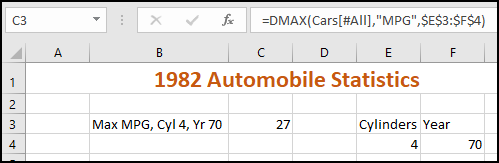
\includegraphics[width=\maxwidth{.95\linewidth}]{gfx/ch09_fig71}
		\caption{Calculating the Max MPG}
		\label{09:fig71}
	\end{figure}
	
	\item Enter \fmtTyping{Avr MPG, Cyl 4, Yr 70} in cell \fmtCellLocation{B4}.
	\item Enter \fmtTyping{=DAVERAGE(Cars[\#All],''MPG'',\$E\$3:\$F\$4)} in cell \fmtCellLocation{C4}.
	\item Excel reports $ 25.28571 $ as the average MPG for $ 1970 $ cars with $ 4 $ cylinders.
	
	\item Enter \fmtTyping{$ 71 $} in \fmtCellLocation{F4}. Notice that Excel automatically updates \fmtCellLocation{C3} and \fmtCellLocation{C4} to reflect the values for $ 1971 $ cars.
	\item Enter \fmtTyping{$ 70 $} in \fmtCellLocation{F4} to change back to that year and match the text in \fmtCellLocation{B3} and \fmtCellLocation{B4}.

	\item Enter \fmtTyping{Avr MPG, Cyl 4-6, Yr 70} in B5.
	\item Enter \fmtTyping{$ 6 $} in \fmtCellLocation{E5} and \fmtTyping{$ 71 $} in \fmtCellLocation{F5}.
	\item Enter \fmtTyping{=DAVERAGE(Cars[\#All],''MPG'',\$E\$3:\$F\$5)} in cell \fmtCellLocation{C5}.
	\item Excel reports $ 23.8 $ as the average MPG for $ 1971 $ cars with $ 4 $ or $ 6 $ cylinders. 
\end{enumerate}	
	
Excel reads the criteria range such that items in a single row are joined with an ``AND'' and multiple rows are joined with an ``OR.'' Thus, the criteria in \fmtCellLocation{E3:F5} reads \textit{(Cars with $ 4 $ cylinders AND year $ 71 $) OR (Cars with $ 6 $ cylinders AND year $ 71 $)}. Very complex Boolean conditions can be specified using multiple rows and columns.

If a cell in a criteria range is empty then Excel matches it to all entries in the data table.

\begin{enumerate}[resume]

	\item Delete the data in \fmtCellLocation{F5}. Notice that the value in \fmtCellLocation{C5} changes to $ 20.94526 $. The criteria in this case reads \textit{(Cars with $ 4 $ cylinders AND year $ 71 $) OR (Cars with $ 6 $ cylinders AND all model years}. 
	\item Enter \fmtTyping{$ 71 $} in \fmtCellLocation{F5}.
	\item Enter \fmtTyping{Origin} in \fmtCellLocation{G3}.
	\item Enter \fmtTyping{American} in \fmtCellLocation{G4}.
	\item Enter \fmtTyping{Avr MPG, Cyl 6, Yr 70, American} in \fmtCellLocation{B6}.
	\item Adjust the width of \fmtCellLocation{Column B} to fit the text in \fmtCellLocation{B6}.
	\item Enter \fmtTyping{=DAVERAGE(Cars[\#All],''MPG'',\$E\$3:\$G\$4)} in cell \fmtCellLocation{C6}.
	\item Excel reports $ 24.75 $ as the average MPG for $ 1971 $ cars with $ 4 $ cylinders made in America. 
	
	\item Complete the summary table using the following information. Adjust the width of \fmtCellLocation{Column B} as necessary to display the text entered there.
	
\end{enumerate}	

\begin{table}[H]
	\rowcolors{1}{}{tablerow} % zebra striping background
	{\small
		%\fontsize{8}{10} \selectfont %Replace small for special font size
		\begin{longtable}{L{0.5in}L{3.50in}} %Left-aligned, Max width: 4.25in
			\textbf{Cell} & \textbf{Content} \endhead
			\hline
			\fmtCellLocation{B7} & \fmtTyping{Max MPG, American}\\
			\fmtCellLocation{C7} & \fmtTyping{=DMAX(Cars[\#All],"MPG",\$G\$3:\$G\$4)}\\

			\fmtCellLocation{F8} & \fmtTyping{Year}\\
			\fmtCellLocation{G8} & \fmtTyping{Origin}\\
			\fmtCellLocation{F9} & \fmtTyping{$ <76 $}\\
			\fmtCellLocation{G9} & \fmtTyping{American}\\
			\fmtCellLocation{B8} & \fmtTyping{Min MPG, Yr<76, American}\\
			\fmtCellLocation{C8} & \fmtTyping{=DMIN(Cars[\#All],"MPG",\$F\$8:\$G\$9)}\\

			\fmtCellLocation{F10} & \fmtTyping{$ <76 $}\\
			\fmtCellLocation{G10} & \fmtTyping{European}\\
			\fmtCellLocation{B8} & \fmtTyping{Avr MPG, Yr<76, American or European}\\
			\fmtCellLocation{C8} & \fmtTyping{=DAVERAGE(Cars[\#All],"MPG",\$F\$8:\$G\$10)}\\
			
			\rowcolor{captionwhite}
			\caption{Information To Complete The Summary Table}
			\label{05:tab01}
		\end{longtable}
	} % End small
\end{table}

The Figure \ref{09:fig72} shows the Summary Table at this point, but it could easily be extended with various combinations of criteria to extract whatever information is desired from the cars data. 

\begin{figure}[H]
	\centering
	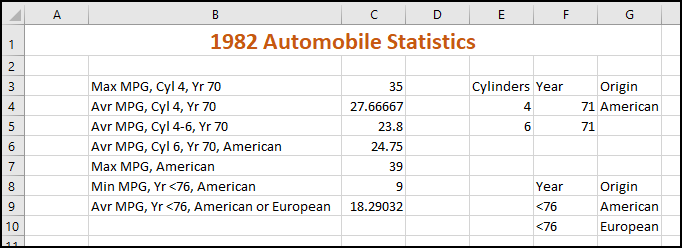
\includegraphics[width=\maxwidth{.95\linewidth}]{gfx/ch09_fig72}
	\caption{Summary Table}
	\label{09:fig72}
\end{figure}


\begin{enumerate}[resume]

	\item Click in \fmtCellLocation{B12} to activate that cell.
	\item Click \fmtRibbonButton{Data $ \Rightarrow $ Analyze $ \Rightarrow $ Data Analysis}.
	\item Select \fmtPopupButton{Correlation} in the \fmtPopupBox{Data Analysis} popup box.
	
	\begin{figure}[H]
		\centering
		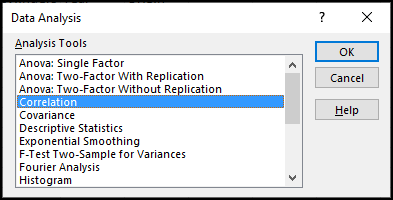
\includegraphics[width=\maxwidth{.95\linewidth}]{gfx/ch09_fig73}
		\caption{Data Analysis Popup}
		\label{09:fig73}
	\end{figure}
	
	\item Enter the following in the \fmtPopupBox{Correlation} popup.
	
	\begin{itemize}
		\item \textbf{Input Range}: \fmtTyping{'Cars'!\$C\$1:\$H\$393}
		\item \textbf{Grouped By}: Columns
		\item \textbf{Labels in first row}: Checked
		\item \textbf{Output Range}: \$B\$12
	\end{itemize}

	\begin{figure}[H]
		\centering
		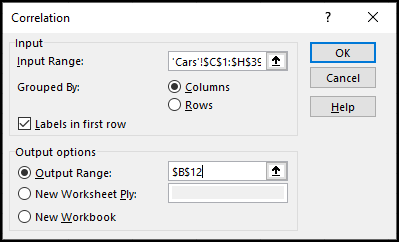
\includegraphics[width=\maxwidth{.95\linewidth}]{gfx/ch09_fig74}
		\caption{Correlation Parameters}
		\label{09:fig74}
	\end{figure}
	
	\item Adjust the column widths so all information in \fmtCellLocation{Row 12} is visible.
	\item Excel calculates the various correlations and displays them in \fmtCellLocation{B12:H18}. There are several rather extreme correlations in the table, but all would be expected. For example, the correlation between weight and MPG is $ -0.83224 $, so heavier cars get fewer miles per gallon.
	
	\begin{figure}[H]
		\centering
		\includegraphics[width=\maxwidth{.95\linewidth}]{gfx/ch09_fig75}
		\caption{Correlation Results}
		\label{09:fig75}
	\end{figure}

	\item Click in \fmtCellLocation{B21} to activate that cell.
	\item Click \fmtRibbonButton{Data $ \Rightarrow $ Analyze $ \Rightarrow $ Data Analysis}.
	\item Select \fmtPopupButton{Histogram} in the \fmtPopupBox{Data Analysis} popup box.
	\item Enter the following in the \fmtPopupBox{Histogram} popup.

	\begin{itemize}
		\item \textbf{Input Range}: \fmtTyping{'Cars'!\$C\$1:\$C\$393}
		\item \textbf{Labels}: Checked
		\item \textbf{Output Range}: \$B\$21
		\item \textbf{Chart Output}: Checked
	\end{itemize}
	
	\begin{figure}[H]
		\centering
		\includegraphics[width=\maxwidth{.95\linewidth}]{gfx/ch09_fig76}
		\caption{Histogram Parameters}
		\label{09:fig76}
	\end{figure}

	\item Excel displays the histogram and chart. 
	\item Adjust the chart so the top left corner is in \fmtCellLocation{D22} and the bottom right corner is in \fmtCellLocation{K38}.
	\item Remove the Chart Elements selector, remove the legend from the histogram.
	\item Change the title of the histogram to \fmtTyping{Car MPG}.
	\item Change the X-Axis title to \fmtTyping{MPG}.

	\begin{figure}[H]
		\centering
		\includegraphics[width=\maxwidth{.95\linewidth}]{gfx/ch09_fig77}
		\caption{Histogram Results}
		\label{09:fig77}
	\end{figure}
	
	\item Save the \fmtWorkbookName{PR9-Cars} workbook and submit it to the instructor.

\end{enumerate}


\section{Scored Assessment}

\subsection{Weather Analysis}

The \textit{National Oceanic and Atmospheric Administration (NOAA)} makes all of their weather data available for researchers to investigate and the data for this exercise was downloaded and adapted from that website \url{https://www.ncdc.noaa.gov/cdo-web/}.

\begin{enumerate}
	\item Open workbook \fmtWorkbookName{SC9-Data}.
\end{enumerate}

This workbook has two worksheets. The \fmtWorksheetName{Data} sheet contains the raw data that will be analyzed for this exercise and the \fmtWorksheetName{Notes} sheet contains definitions for the abbreviations used on the \fmtWorksheetName{Data} sheet.

\begin{enumerate}[resume]
	\item Save the workbook as \fmtWorkbookName{SC9-Climate}.
	\item Calculate the number of hours of daylight for each day.
	
	\begin{enumerate}
		\item Insert a new column to the left of \fmtCellLocation{Column N}.
		\item Enter \fmtTyping{Daylight} in cell \fmtCellLocation{N1}.
		\item Enter \fmtTyping{=M2-L2} in cell \fmtCellLocation{N2}.
		\item Copy/paste \fmtCellLocation{N2} to \fmtCellLocation{N3:N363}.
	\end{enumerate}
	
	\item Convert the data to a table.
	
	\begin{enumerate}
		\item Click in \fmtCellLocation{A1} to activate that cell.
		\item Click \fmtRibbonButton{Insert $ \Rightarrow $ Tables $ \Rightarrow $ Table}.
		\item Excel will automatically select the entire data set, \fmtCellLocation{\$A\$1:\$O\$363}. Be sure \fmtPopupButton{My table has headers} is checked.
		\item Click \fmtPopupButton{OK}.
		\item Name the table \fmtTyping{Climate}.
	\end{enumerate}
	
	\begin{figure}[H]
		\centering
		\includegraphics[width=\maxwidth{.95\linewidth}]{gfx/ch09_fig85}
		\caption{Climate Table Name}
		\label{09:fig85}
	\end{figure}
	
	\item Create a new worksheet and name it \fmtTyping{Summary}.
	\item Move \fmtWorksheetName{Summary} to the left of \fmtWorksheetName{Data} so it is the first worksheet in the workbook.
	\item Click the \fmtWorksheetName{Summary} tab to activate that sheet.
	\item Select \fmtCellLocation{A1:G1} and click \fmtPopupButton{Merge \& Center}.
	\item Enter \fmtTyping{2019 Ft Huachuca Climate Information} in cell \fmtCellLocation{A1}.
	\item Format cell \fmtCellLocation{A1}.
	
		\begin{itemize}
			\item Calibri font, 18 pt
			\item Bold style
			\item Font color: Blue, Accent 1
		\end{itemize}

	\item Enter \fmtTyping{Date} in cell \fmtCellLocation{B3}. (Note: this will be the starting date for formulas on this sheet, but the title in \fmtCellLocation{B3} must match the field name on the Climate table.)
	\item Enter \fmtTyping{Date} in cell \fmtCellLocation{C3}. (Note: this will be the ending date for formulas on this sheet, but the title in \fmtCellLocation{C3} must match the field name on the Climate table.)
	\item Enter \fmtTyping{Max Temp} in cell \fmtCellLocation{B5}.
	\item Enter \fmtTyping{$ >=1/1/2019 $} in cell \fmtCellLocation{B4}.
	\item Enter \fmtTyping{$ <=1/31/2019 $} in cell \fmtCellLocation{C4}.
	\item Adjust the width of \fmtCellLocation{Column B} and \fmtCellLocation{Column C} so everything is visible.
	\item Enter this formula into \fmtCellLocation{C5}: \fmtTyping{=DMAX(Climate[\#All],''TMAX'',\$B\$3:\$C\$4)}.
	\item Cell \fmtCellLocation{C5} will display $ 72 $, which is the greatest \textit{TMAX} for January, $ 2019 $.

	\begin{figure}[H]
		\centering
		\includegraphics[width=\maxwidth{.95\linewidth}]{gfx/ch09_fig86}
		\caption{Maximum January Temperature}
		\label{09:fig86}
	\end{figure}

	\item Change the dates to \fmtTyping{$ >=3/1/2019 $} and \fmtTyping{$ <=3/31/2019 $} to find that the maximum March temperature is $ 82 $.
	\item Change the dates back to \fmtTyping{$ >=1/1/2019 $} and \fmtTyping{$ <=1/31/2019 $} to complete the other activities on the summary sheet.

	\item Enter \fmtTyping{Min Temp} into \fmtCellLocation{B6}.
	\item Enter this formula into \fmtCellLocation{C6}: \fmtTyping{=DMIN(Climate[\#All],''TMIN'',\$B\$3:\$C\$4)}.
	\item Cell \fmtCellLocation{C6} will display $ 21 $, which is the least \textit{TMIN} for January, $ 2019 $.

	\item Enter \fmtTyping{Precitation} into \fmtCellLocation{B7}.  (The width of \fmtCellLocation{Column B} may need to be changed to see the word \textit{Precipitation}.)
	\item Enter this formula into \fmtCellLocation{C7}: \fmtTyping{=DSUM(Climate[\#All],''PRCP'',\$B\$3:\$C\$4)}.
	\item Cell \fmtCellLocation{C7} will display $ 0.9 $, which is the total precipitation for January, $ 2019 $.

	\item Enter \fmtTyping{Wind Speed} into \fmtCellLocation{B8}.
	\item Enter this formula into \fmtCellLocation{C8}: \fmtTyping{=DAVERAGE(Climate[\#All],''AWND'',\$B\$3:\$C\$4)}.
	\item Cell \fmtCellLocation{C8} will display $ 8.002258065 $, which is the average wind speed for January, $ 2019 $.
	\item To make \fmtCellLocation{C8} easier to read, click \fmtRibbonButton{Home $ \Rightarrow $ Number $ \Rightarrow $ Decrease Decimal} to reduce \fmtCellLocation{C8} to $ 8.00 $.

	\item Enter \fmtTyping{Max Wind} into \fmtCellLocation{B9}.
	\item Enter this formula into \fmtCellLocation{C9}: \fmtTyping{=DMAX(Climate[\#All],''WSF5'',\$B\$3:\$C\$4)}.
	\item Cell \fmtCellLocation{C9} will display $ 42.90 $, which is the greatest wind gust for January, $ 2019 $.

	\item Copy/paste \fmtCellLocation{B3:C4} to \fmtCellLocation{B11:C12}.
	\item Enter \fmtTyping{Moon} into \fmtCellLocation{D11}.
	\item Enter \fmtTyping{New} into \fmtCellLocation{D12}.
	\item Enter \fmtTyping{$ <= 12/31/2019 $} into \fmtCellLocation{C12}.
	\item Enter \fmtTyping{Coldest New Moon} into \fmtCellLocation{B13}. (The width of \fmtCellLocation{Column B} may need to be changed to see the words \textit{Coldest New Moon}.)
	\item Enter this formula into \fmtCellLocation{C13}: \fmtTyping{=DMIN(Climate[\#All],''TMIN'',\$B\$3:\$D\$4)}.
	\item Cell \fmtCellLocation{C13} will display $ 32 $, which was the coldest temperature recorded on a night with a new moon in $ 2019 $.

	\item Copy/paste \fmtCellLocation{B11:D12} to \fmtCellLocation{B15:D16}.
	\item Enter \fmtTyping{DailyWeather} into \fmtCellLocation{D15}.
	\item Enter \fmtTyping{*TS*} into \fmtCellLocation{16}. Note: the asterisks are ``wildcard'' characters and will create a match on any cell that contains \textit{TS} somewhere in the cell.
	\item Enter \fmtTyping{Largest Storm} into \fmtCellLocation{B17}.
	\item Enter this formula into \fmtCellLocation{C17}: \fmtTyping{=DMAX(Climate[\#All],''PRCP'',\$B\$3:\$D\$4)}.
	\item Cell \fmtCellLocation{C17} will display $ 2.32 $, which was the most rainfall on a day that recorded thunder in $ 2019 $.
	
	\begin{figure}[H]
		\centering
		\includegraphics[width=\maxwidth{.95\linewidth}]{gfx/ch09_fig87}
		\caption{Various Summary Statistics}
		\label{09:fig87}
	\end{figure}
	
\end{enumerate}	

Next, create a chart that shows the amount of daylight throughout the year. (Note: the process for creating charts is covered in more detail in Chapter \ref{ch04:charts}, page \pageref{ch04:charts}.)

\begin{enumerate}
	\item Activate the \fmtWorksheetName{Data} worksheet.
	\item Activate \fmtCellLocation{Column N} by clicking the top of the column.
	\item Click \fmtRibbonButton{Insert $ \Rightarrow $ Charts $ \Rightarrow $ Insert Line or Area Chart}.
	\item In the \fmtPopupBox{Line Chart} popup, select the first option, \fmtPopupButton{2-D Line}.
	\item Excel will create a line chart that shows the amount of daylight throughout the year. 
	
	\begin{figure}[H]
		\centering
		\includegraphics[width=\maxwidth{.95\linewidth}]{gfx/ch09_fig88}
		\caption{Daylight Chart: Start}
		\label{09:fig88}
	\end{figure}
	
	\item Right-click the chart and select \fmtPopupButton{Move Chart}. Move it as an object in the \fmtWorksheetName{Summary} worksheet.

	\begin{figure}[H]
		\centering
		\includegraphics[width=\maxwidth{.95\linewidth}]{gfx/ch09_fig89}
		\caption{Daylight Chart: Moving to Summary Worksheet}
		\label{09:fig89}
	\end{figure}

	\item Drag/drop the chart so the top-left corner is about in cell \fmtCellLocation{B20}.
	\item By default, the horizontal axis simply counts the number of entries from $ 1 $ to $ 363 $, but it should display the dates found in \fmtCellLocation{Column A}.
	\item Click the chart area to display the three buttons on the right side of the chart. Click the \fmtPopupButton{Chart Filters} button, which looks like a funnel.
	
	\begin{figure}[H]
		\centering
		\includegraphics[width=\maxwidth{.95\linewidth}]{gfx/ch09_fig90}
		\caption{Daylight Chart: Chart Filters}
		\label{09:fig90}
	\end{figure}

	\item Notice that the Categories filter is just a list of numbers, starting at one. Click the \fmtPopupButton{Select Data} button at the bottom of the \fmtPopupBox{Values} popup box. The \fmtPopupBox{Select Data Source} popup box appears.

	\begin{figure}[H]
		\centering
		\includegraphics[width=\maxwidth{.95\linewidth}]{gfx/ch09_fig91}
		\caption{Daylight Chart: Select Data Source}
		\label{09:fig91}
	\end{figure}
	
	\item Click \fmtPopupButton{Edit} for the \fmtPopupBox{Horizontal (Category) Axis Labels}. That button is marked in Figure \ref{09:fig91}.
	\item Enter \fmtTyping{=Data!\$A\$2:\$A\$363} for the Axis label range.
	
	\begin{figure}[H]
		\centering
		\includegraphics[width=\maxwidth{.95\linewidth}]{gfx/ch09_fig92}
		\caption{Daylight Chart: Axis Labels}
		\label{09:fig92}
	\end{figure}
	
	\item Excel changes the labels for the X-Axis to the dates found in \fmtCellLocation{Column A} of the \fmtWorksheetName{Data} worksheet. Click \fmtPopupButton{OK} on the \fmtPopupBox{Select Data Source} popup box to finish this selection.
	\item To adjust the scale for the Y-Axis (the hours of daylight), right-click on the vertical axis values and select \fmtPopupButton{Format Axis}.
	\item In the \fmtPopupBox{Format Axis} popup, enter \fmtTyping{$ 0.35 $} for the \fmtPopupBox{Minimum Bounds} (the \fmtPopupBox{Maximum Bounds} will automatically adjust).
	
	\begin{figure}[H]
		\centering
		\includegraphics[width=\maxwidth{.95\linewidth}]{gfx/ch09_fig93}
		\caption{Daylight Chart: Adjusting Y-Axis Scale}
		\label{09:fig93}
	\end{figure}
	
	\item Submit the \fmtWorkbookName{SC-Climate} workbook to the instructor.
\end{enumerate}





	


